\section{模型构建与分析}

\subsection{LSTM长短时记忆网络}
\label{subsec:lstm}

\subsubsection{算法介绍}

LSTM(Long Short-Term Memory Networks,长短时记忆网络),由Hochreiter和Schmidhuber于1997年提出 \cite{LSTM_Hochrerter},目的是解决一般循环神经网络中存在的梯度爆炸(输入信息激活后权重过小)及梯度消失(例如sigmoid、tanh的激活值在输入很大时其梯度趋于零)问题,主要通过引入门和Cell状态的概念来实现梯度的调整。LSTM采用了门控输出的方式,即三门(输入门、遗忘门、输出门)两态(Cell State长时、Hidden State短时)。其核心即Cell State,指用于信息传播的Cell的状态,其结构示意图如图 \ref{fig:a-0}所示:

\begin{figure}[ht]
  \centering
  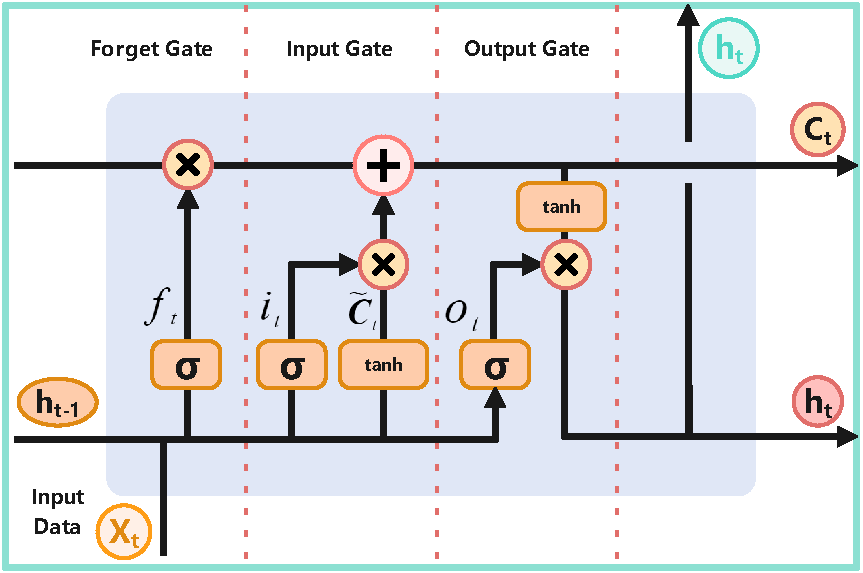
\includegraphics[width=0.65\textwidth]{./Img/LSTM解释结构图.pdf}
  \caption{LSTM详细结构图}\label{fig:a-0}
\end{figure}


\subsubsection{数据预处理}

在开展气象预测模型的研究过程中,我们选取了从2015年2月至2016年8月期间的气象记录作为研究样本。此数据集不仅包含了日期基本信息(年、月、日),还涵盖了日均温、日最低温、日最高温、相对湿度、风速和降水量等多个关键气象参数。

\begin{table}[!ht]
    \caption{2015年2月-2016年8月期间的有效气象数据}\label{tab:LSTM_data}
    \centering
    \resizebox{1.0\linewidth}{!}
    {\begin{threeparttable} 
    \begin{tabular}{*9{c}}\toprule
        序号 & 年份 & 月份 & 日号 & 日最高气温\tnote{1} & 日最低气温\tnote{1} & 日平均气温\tnote{1}  & 相对湿度($\%RH$) & 降水量($mm$) \\  
        \midrule
        1 & 2015 & 2 & 1 & 1.9 & -0.4 & 0.7875 & 75.000 & 160.477961 \\ 
        2 & 2015 & 2 & 2 & 6.2 & -3.9 & 1.7625 & 77.250 & 129.268657 \\ 
        3 & 2015 & 2 & 3 & 7.8 & 2.0 & 4.2375 & 72.750 & 107.316539 \\ 
        4 & 2015 & 2 & 4 & 8.5 & -1.2 & 3.0375 & 65.875 & 132.549075 \\ 
        5 & 2015 & 2 & 5 & 7.9 & -3.6 & 1.8625 & 55.375 & 91.082841 \\ 
        $\cdots$ & $\cdots$ & $\cdots$ & $\cdots$ & $\cdots$ & $\cdots$ & $\cdots$ & $\cdots$ & $\cdots$ \\ 
        576 & 2016 & 8 & 29 & 29.9 & 18.1 & 23.7125 & 62.500 & 283.897344 \\ 
        577 & 2016 & 8 & 30 & 29.3 & 16.9 & 23.3250 & 71.500 & 299.212180 \\ 
        578 & 2016 & 8 & 31 & 30.4 & 18.6 & 24.5250 & 68.750 & 292.517916 \\
        \bottomrule
    \end{tabular}    
    \begin{tablenotes}    
        \small              
        \item[1] 气温单位:${}^{\circ}\text{C}$
    \end{tablenotes}          
    \end{threeparttable}}
    \vspace{-0.8em}
\end{table}


在数据预处理阶段,针对数据集中出现的缺失值和异常值,我们选择在该数据集中采取了向前取该时间序列中可用数据的均值进行填补的策略,并剔除了缺失超过三项气象指标的数据,以确保分析的严谨性。经过这一系列处理后,最终得到了共计578条有效气象观测数据,整理后的有效数据如表 \ref{tab:LSTM_data} 所示。



\subsubsection{模型建立}\label{subsubsec:lstm_model_build}

在LSTM中,Memory Cell接受两个输入,即上一时刻的输出值 $h_{t-1}$ 和本时刻的输入值 $X_t$ ,由这两个参数先进入遗忘门,得到决定要舍弃的信息 $f_{t}$ 后,再进入输入门,得到要更新的信息 $i_t$ 和当前时刻的Cell状态 $\widetilde{C}_t$ ,最后由遗忘门与输入门的输出值(即 $f_t$,$X_t$,$\widetilde{C}_t$)进行组合,组合的计算公式如下所示:
\begin{align}
    h_t = C^{t-1} \times f_t \times \widetilde{C}_t \times i_t
\end{align}

其中,$C^{t-1}$表示上一时刻的Cell状态,$f_t$ 为遗忘信息的激活值,$\widetilde{C}_t$ 为当前时刻Cell状态,$i_t$ 表示当前时刻需要记忆信息的激活值,得到分别的长时 $C_t$ 和短时 $h_t$ 信息,最后进行存储操作及对下一个神经元的输入。因此,LSTM在网络中的工作流程如下图所示:


\begin{figure}[ht]
  \centering
  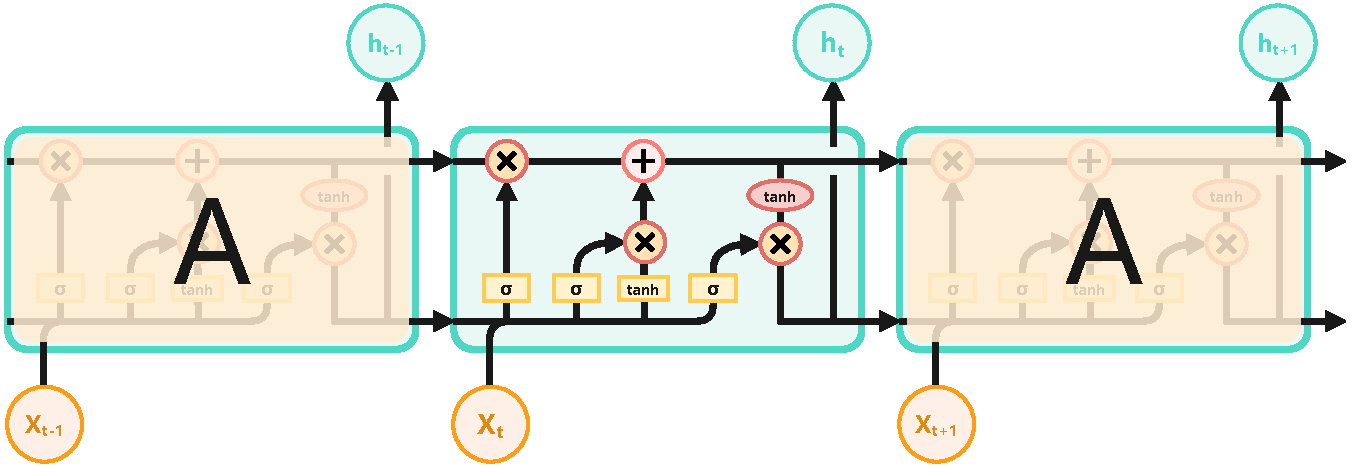
\includegraphics[width=0.9\textwidth]{./Img/LSTM工作流程图.pdf}
  \caption{LSTM工作流程图}\label{fig:aa-2}
\end{figure}

如图 \ref{fig:aa-2} 所示,可以看到LSTM在处理时序数据时的内部运作机制。它通过输入门、遗忘门和输出门的控制以及细胞状态的更新,能够有效地捕捉和利用时间序列数据中的长时依赖关系,从而提供更准确的序列模型以及预测效果。由此可依次得到遗忘门、输入门与输出门的形式方程如下:

\begin{enumerate}
    \item \textbf{遗忘门}:对于上一个时刻Cell输出的 $h_{t-1}$,结合遗忘门的权重矩阵 $W_f$ 与偏置项 $b_f$,综合处理后得到 $t$ 时刻的遗忘门的计算公式如下:
    \begin{align}
        f_t=\sigma(W_f\cdot[h_{t-1},X_t]+b_f)
    \end{align}

    \item \textbf{输入门}:输入层的信息的数量 $i$ 与Cell状态信息 $C$ 在 $t$ 时刻的计算公式如下:
    \begin{align}
        i_t &= \sigma(W_i\cdot[h_{t-1},X_t]+b_i) \label{eq:ea_1}\\
        \widetilde{C}_t &= \tanh(W_c\cdot[h_{t-1},X_t]+b_i) \label{eq:ea_2}
    \end{align}
    其中,$\sigma(\cdot)$ 与 $\tanh(\cdot)$ 分别为Sigmoid激活函数和 $\tanh$ 激活函数,$t$ 为总时间数,$t=0,1,2,\dots,T$。因此,结合公式(\ref{eq:ea_1})和公式(\ref{eq:ea_2}),得到 $t$ 时刻的Cell状态(长时)方程为:
    \begin{align}
        C_t=f_t\cdot C_{t-1}+i_t\cdot\widetilde{C}_t
    \end{align}

    \item \textbf{输出门}:
    \begin{align}
        o_t = &\sigma(W_o\cdot[h_{t-1},X_t]+b_o) \\
        &h_t = o_t\cdot\tanh(C_t)   \label{eq:ea_01}
    \end{align}
    其中,$\tanh(\cdot)$ 具体的计算公式如下:
    \begin{align}
        \tanh(z) &= \frac{e^z-e^{-z}}{e^z+e^{-z}} \\
        \tanh^{\prime}(z) &= 1-\tanh^2(z)
    \end{align}
\end{enumerate}
经过上面的计算,得到了遗忘门、输入门和输出门这三个门的形式方程,可以进一步计算得到下面的前向传播公式:

\textbf{遗忘门:}遗忘门的输出依赖三个变量,分别是上一时刻 $(t-1)$ 神经元的短时记忆输出 $h_{t-1}$,本时刻 $(t)$ 神经元的输入 $X_t$ 以及上一时刻 $(t-1)$ 神经元的长时记忆输出Cell状态 $s^{t-1}_{c}$,乘以权重因子后对层数求和即可的到遗忘门的输入值以及激活值,公式表示如下:
\begin{align}
    a_\phi^t = \sum_{i=1}^lW^{i}_{\phi} \cdot X_i^t+&\sum_{h=1}^HW^{h}_{\phi} \cdot b_h^{t-1}+\sum_{c=1}^CW^{c}_{\phi} \cdot s_c^{t-1} \label{eq:ea_3}\\
    &b_\phi^t = f(a_\phi^t) \label{eq:ea_4}
\end{align}

在公式(\ref{eq:ea_3})和公式(\ref{eq:ea_4})中,$b_\phi^t$ 表示 $t$ 时刻第 $\phi$ 个单元的激活值,在 $t=0$ 时,初始化为 $0$;$a_j^t$ 表示 $t$ 时刻第 $j$ 个单元带权输入;$s_c^{t-1}$ 表示 $t$ 时刻记忆元胞 $c$ 的状态。

\textbf{输入门:}输入门的输入所依赖的变量与遗忘门相同,因此与遗忘门前向传播同理,对于每一个LSTM单元的输入门 $l$,可以得到如下计算公式:
\begin{align}
    a_l^t=\sum_{i=1}^IW^i_{l} \cdot X_i^t+&\sum_{h=1}^HW^h_{l} \cdot b_h^{t-1}+\sum_{c=1}^CW^c_{l} 
\cdot s_c^{t-1} \\
    &b_l^t=f(a_l^t)
\end{align}




\textbf{Cell状态:}根据公式(\ref{eq:ea_1})和公式(\ref{eq:ea_2})中关于输入门 $t$ 时刻的Cell状态方程设定,可得Cell的状态计算公式如下:
\begin{align}
    a_c^t=\sum_{i=1}^lW^i_{c} \cdot X_i^t+\sum_{h=1}^HW^h_{c} \cdot b_h^{t-1}
\end{align}
其中,$c$ 表示一个神经元中的某一个 $C$ 记忆元胞。针对 $s_c^t$ 结合 $C_t$ 的原始公式采用对应的形式方程转换,得到$s^t_c$ 的表达式如下:
\begin{align}
    &\text{形式式:} C_t = f_t\cdot C_{t-1}+ i_t\cdot\widetilde{C}_t \\
    &\text{转换式:} s_c^t = b_\phi^t\cdot s_c^{t-1} + b_l^t\cdot g(a_c^t) 
\end{align}
上式中,$g(\cdot)$ 为Cell输出的激活函数。

\textbf{输出门:}与遗忘门输出公式同理,对于每个LSTM单元的输出门 $w$,可得到输出门计算公式:
\begin{align}
    a_\omega^t=\sum_{i=1}^IW^i_{\omega} \cdot X_i^t+&\sum_{h=1}^HW^h_{\omega} \cdot b_h^{t-1}+\sum_{c=1}^CW^c_{\omega} \cdot s_c^{t-1} \\
    &b_\omega^t=f(a_\omega^t)
\end{align}

\textbf{Cell输出:}激活后的Cell状态(短时记忆),同理可由公式(\ref{eq:ea_01})通过形式方程转换得到 $b^t_c$,其计算公式如下:
\begin{align}
    &\text{形式式:} h_t = o_t\cdot \tanh(C_t) \\
    &\text{转换式:} b_c^t = b_\omega^t \cdot \tanh(s_c^t)
\end{align}


\subsubsection{实验结果}


经过数据预处理环节之后,有效的气象数据集如表 \ref{tab:LSTM_data} 所示。在作为模型的输入数据之前,所有数据集需要进行数据归一化,归一化的计算方法如下:
\begin{align}
    y = \frac{x_i-x_{min}}{x_{max}-x_{min}}
\end{align}


\begin{table}[!ht]
    \caption{归一化后的气象数据}\label{tab:LSTM_data——normalization}
    \centering
    \resizebox{1.0\linewidth}{!}
    {\begin{threeparttable}          %这行要添加
    \begin{tabular}{*9{c}}\toprule
        序号 & 年份 & 月份 & 日号 & 日最高气温\tnote{1} & 日最低气温\tnote{1} & 日平均气温\tnote{1}  & 相对湿度($\%RH$) & 降水量($mm$) \\ 
        \midrule
        1 & 2015 & 2 & 1 & 0.04986877 & 0.26582278 & 0.2126935 & 0.59916493 & 0.12233463 \\ 
        2 & 2015 & 2 & 2 & 0.16272966 & 0.17721519 & 0.23684211 & 0.63674322 & 0.09633772 \\ 
        3 & 2015 & 2 & 3 & 0.20472441 & 0.32658228 & 0.29814241 & 0.56158664 & 0.07805192 \\ 
        4 & 2015 & 2 & 4 & 0.22309711 & 0.24556962 & 0.26842105 & 0.44676409 & 0.09907027 \\ 
        5 & 2015 & 2 & 5 & 0.20734908 & 0.18481013 & 0.23931889 & 0.27139875 & 0.06452948 \\ 
        $\cdots$ & $\cdots$ & $\cdots$ & $\cdots$ & $\cdots$ & $\cdots$ & $\cdots$ & $\cdots$ & $\cdots$ \\ 
        576 & 2016 & 8 & 29 & 0.7847769 & 0.73417722 & 0.78049536 & 0.39039666 & 0.22514122 \\ 
        577 & 2016 & 8 & 30 & 0.76902887 & 0.70379747 & 0.77089783 & 0.54070981 & 0.23789826 \\ 
        578 & 2016 & 8 & 31 & 0.79790026 & 0.74683544  & 0.8006192 & 0.49478079 & 0.23232203 \\ 
        \bottomrule
    \end{tabular}
    \begin{tablenotes}    
        \small              
        \item[1] 气温单位:${}^{\circ}\text{C}$
    \end{tablenotes}          
    \end{threeparttable}}
    \vspace{-0.8em}
\end{table}

\begin{figure}[ht]
  \centering
  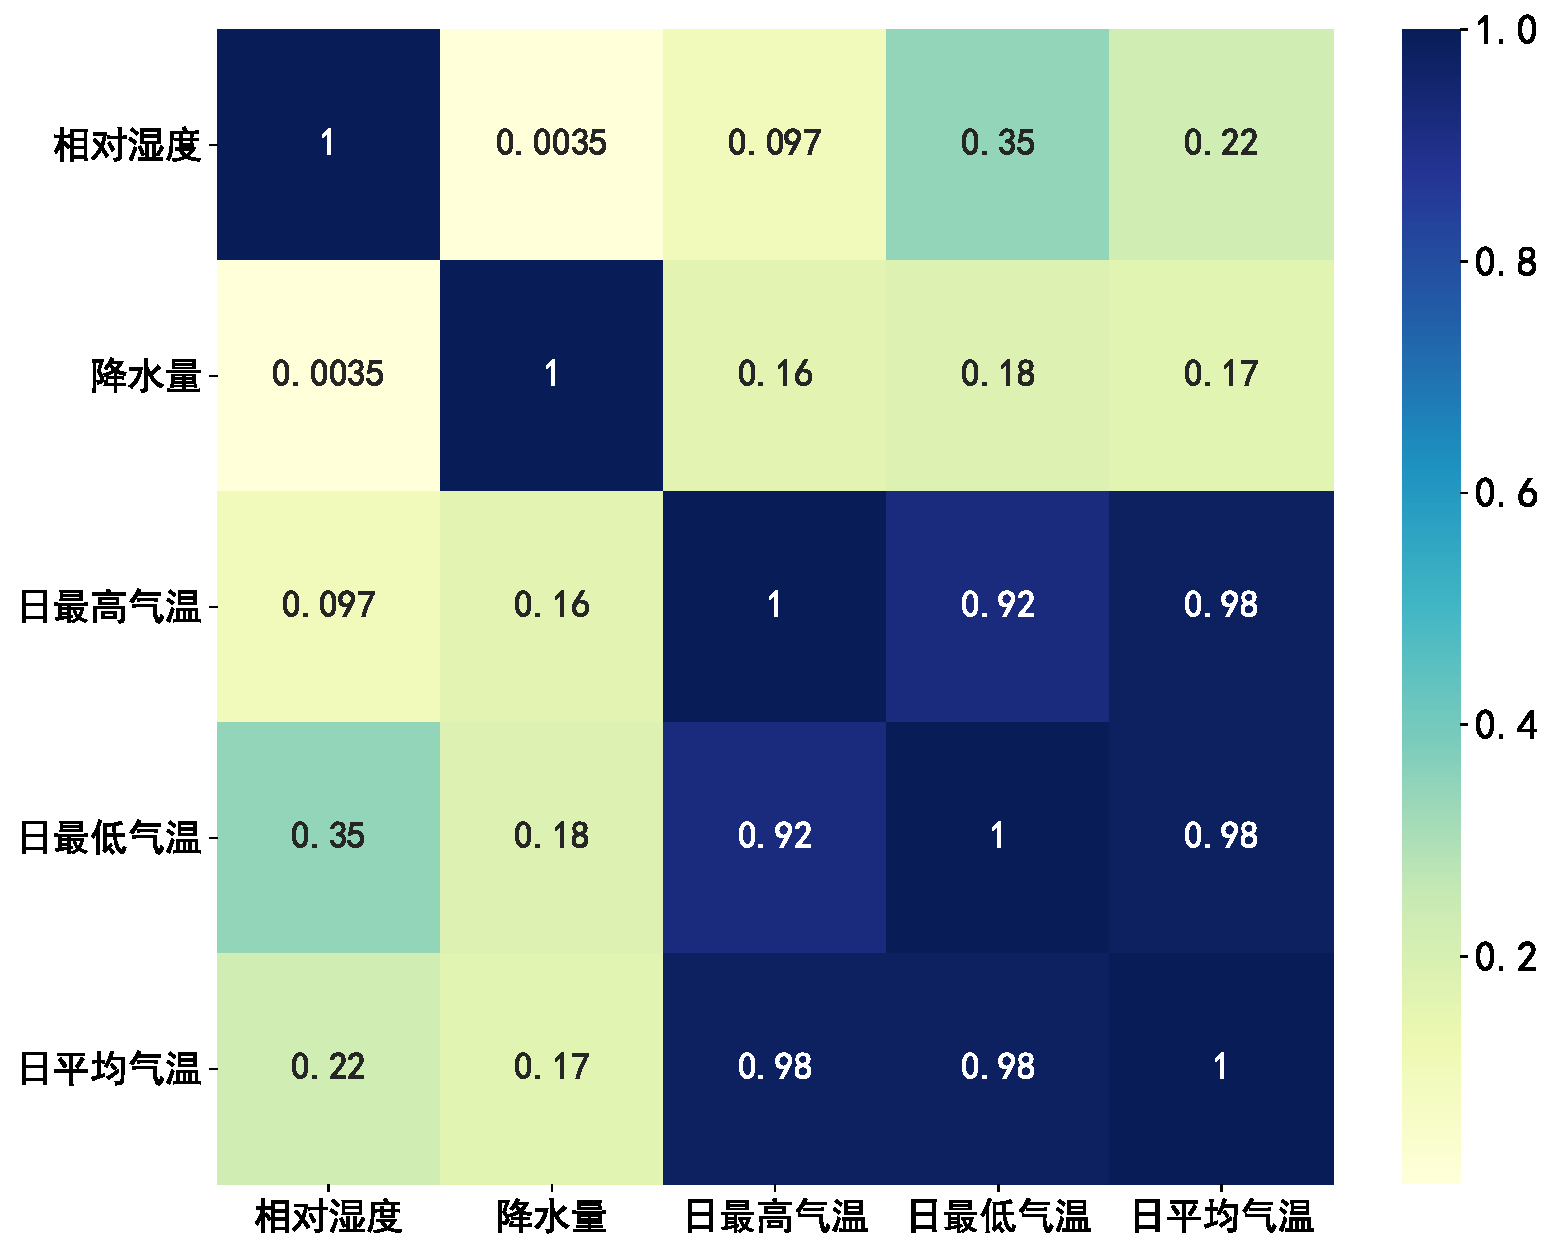
\includegraphics[width=0.7\textwidth]{./Img/相关性热力图.pdf}
  \caption{有效数据中不同指标间的相关性热力图}\label{fig:4-7-a}
\end{figure}

\begin{figure}[ht]
  \centering
  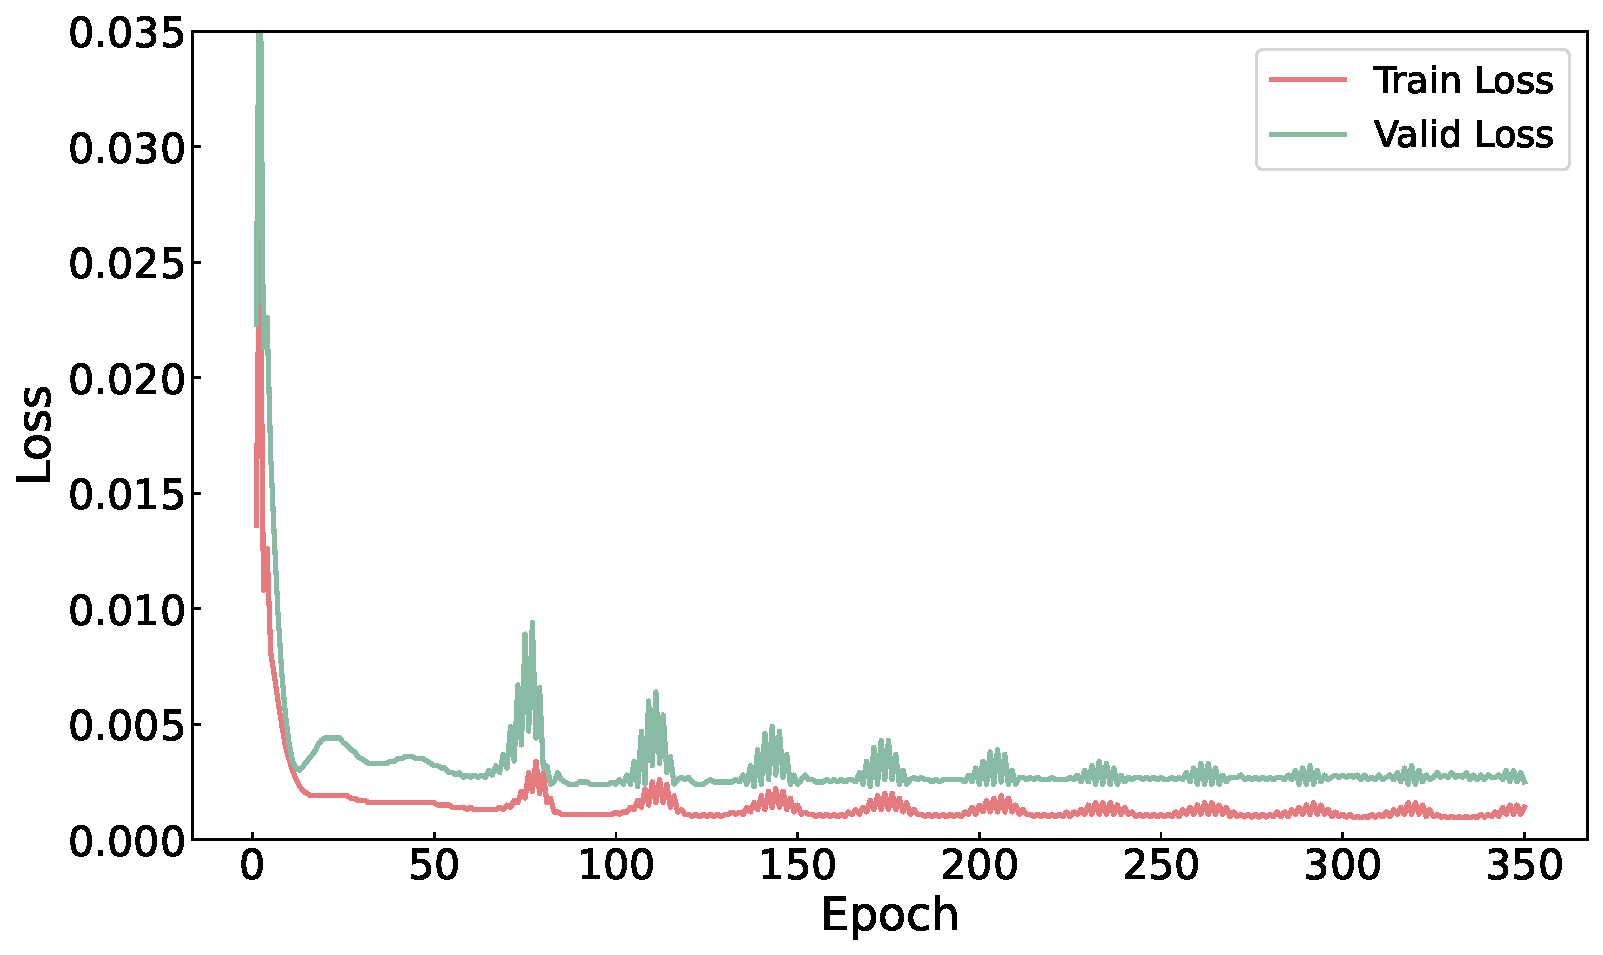
\includegraphics[width=0.7\textwidth]{./Img/LSTM_loss.pdf}
  \caption{LSTM模型的训练损失和验证损失}\label{fig:4-7}
\end{figure}

\begin{figure}[t]
  \centering
  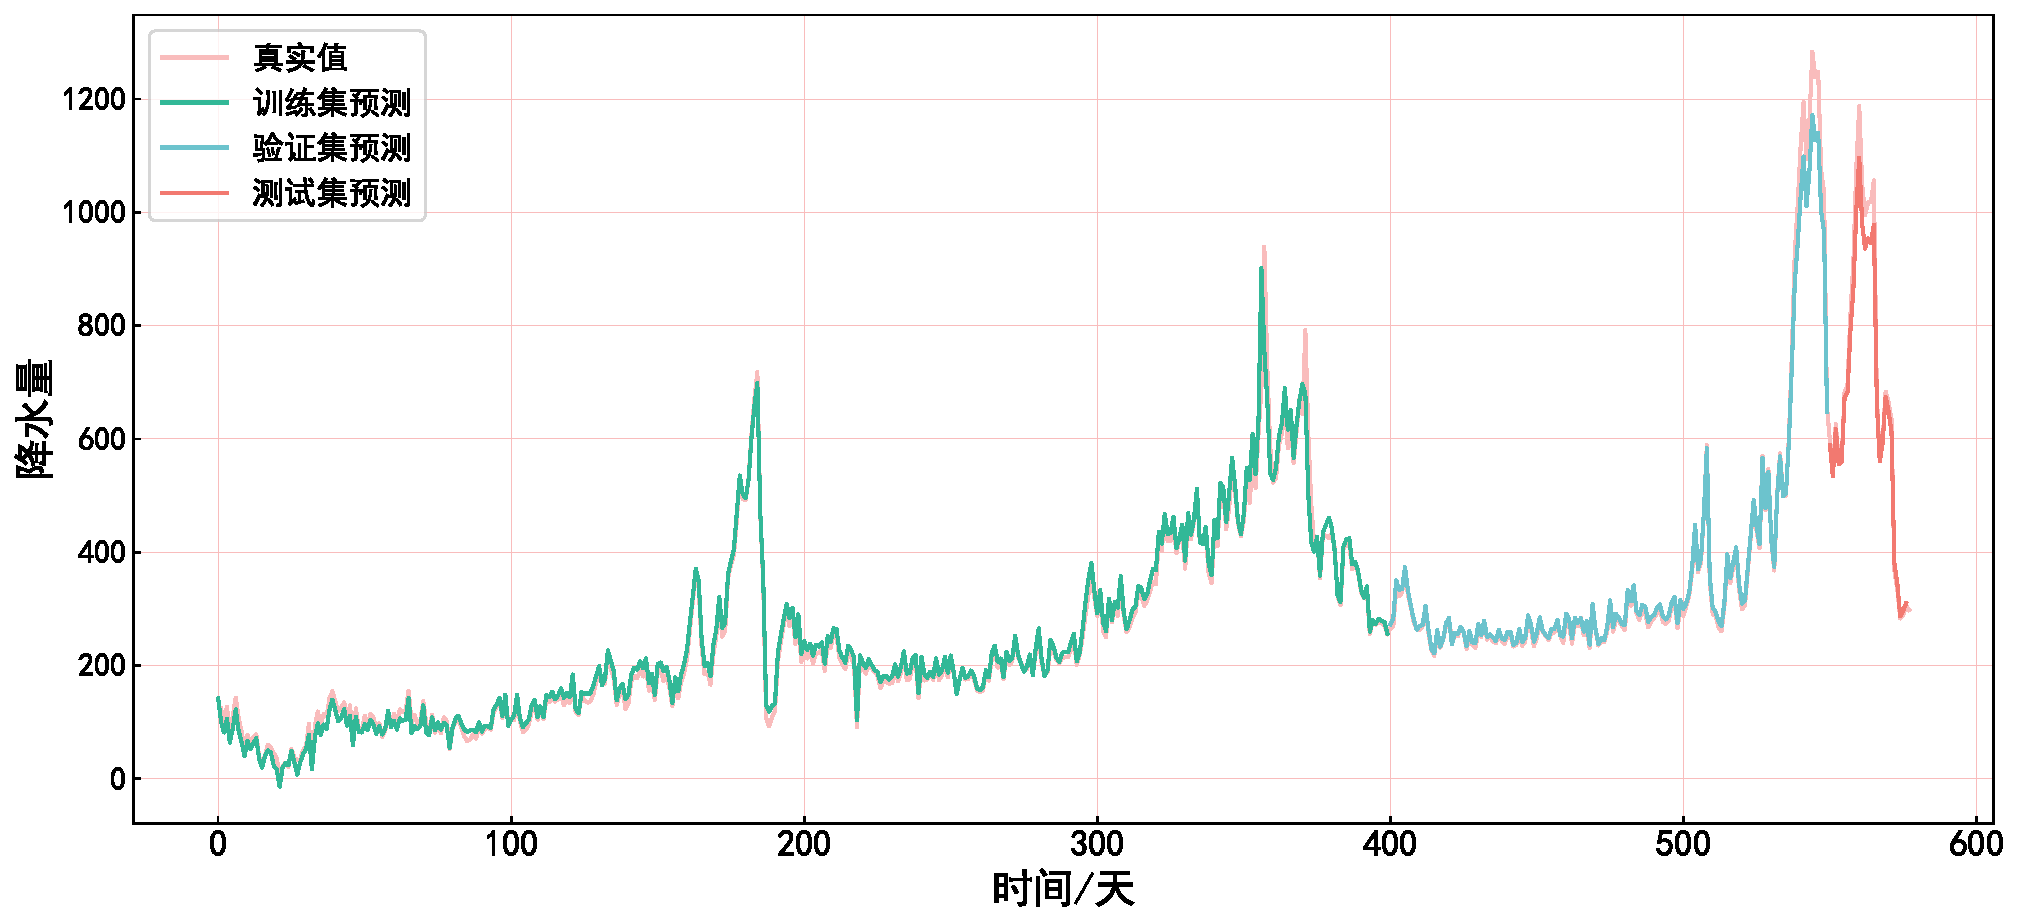
\includegraphics[width=1.0\textwidth]{./Img/LSTM_pre.pdf}
  \caption{LSTM模型针对三个数据集的预测结果}\label{fig:4-8}
\end{figure}

\begin{figure}[h]
  \centering
  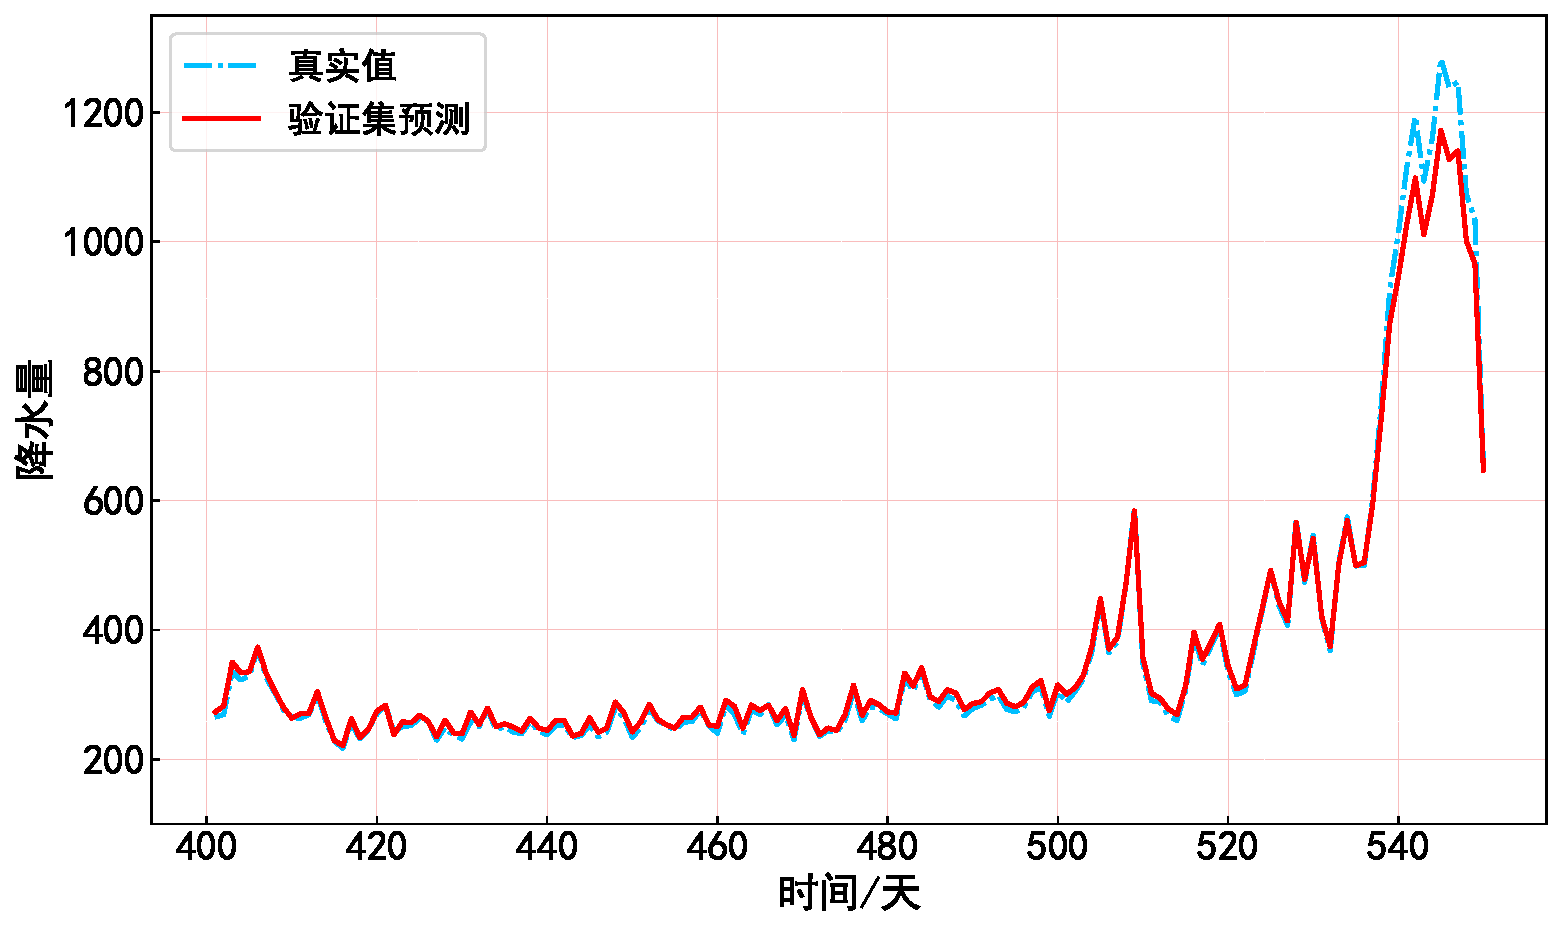
\includegraphics[width=0.7\textwidth]{./Img/LSTM_valid_pre.pdf}
  \caption{验证集预测结果与真实值对比}\label{fig:4-9}
\end{figure}

\begin{figure}[h]
  \centering
  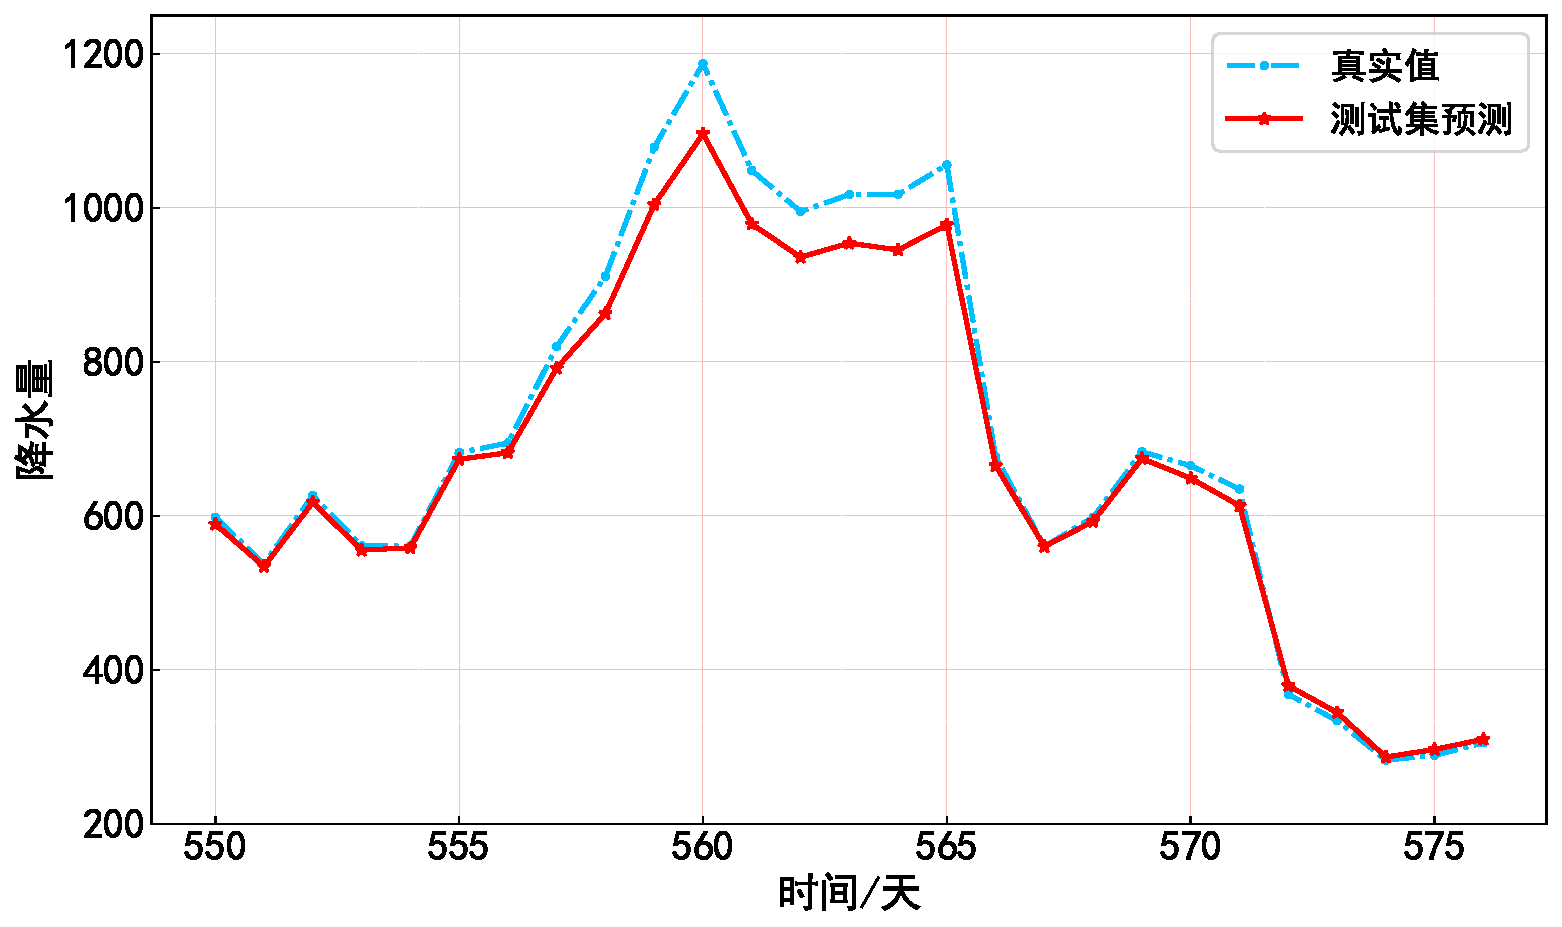
\includegraphics[width=0.7\textwidth]{./Img/LSTM_test_pre.pdf}
  \caption{测试集预测结果与真实值对比}\label{fig:4-10}
\end{figure}


如表 \ref{tab:LSTM_data——normalization} 得到归一化后的数据集之后,我们首先对日最高气温、日最低气温、日平均气温、相对湿度以及降水量组成的五个指标的特征集计算了相关性,得到的相关性的热力图如图 \ref{fig:4-7-a} 所示。观察图 \ref{fig:4-7-a} 可以看出,降水量与相对湿度的相关性微乎其微,仅0.0035,而与日最高气温、日最平均气温和日最低气温的相关性逐渐提升,但仍属中低水平,相关系数在0.16至0.18范围内。

值得注意的是,日最高气温、日最平均气温和日最低气温这三个指标由于属性相近和受到影响相同,因此彼此间存在极高相关性。整体上这些指标间展现了一种平衡状态,既体现了适度的相关性也保持了某种程度的互斥性,具备了一定的随机性,可以提高模型的泛化性能。

接下来,我们按照天数来划分训练集、测试集以及验证集,经过多次实验的测试,对不同的实验结果综合分析之后,选出了较优的划分区间,针对总共578天的数据,训练集我们选择 $[1,400]$ 这个天数区间作为训练,选择 $[401,549]$ 这个天数区间作为验证集,最后的 $[550,578]$ 这个区间作为测试集。在上一小节中,我们建立了LSTM模型,以降水量作为输出值,设定训练时epoch次数为350次,隐含层神经元的个数为1024个,训练时的每一批量大小为16,采用ReLU和Adam分别作为激活函数和优化器,经过上述的实验前提设定后,模型正式进入训练阶段,训练阶段的训练时损失和验证时损失如图 \ref{fig:4-7} 所示。训练完成后,使用训练好的模型分别针对训练集、验证集以及测试集进行模型推理,并将三个部分数据合并到一块,为了使各个部分有一定的区分,我们给训练集、验证集和测试集的预测结果以及真实值分别设置了不同的颜色,得到的结果如图 \ref{fig:4-8} 所示。

为清晰呈现验证集与测试集的预测效能,我们抽离了两者的数据,并分别在图 \ref{fig:4-9} 及图 \ref{fig:4-10} 中直观显现。从图中可以看出,在预测降水量方面,验证集的预测值与实测数据之间展现出高度吻合,有力证明了模型在此预测指标上的精确度。进一步深化对模型性能的分析,我们利用已训练完成的模型对[550, 575]天数范围内的数据进行了预测。预测结果的详细数据展示在表 \ref{tab:LSTM_data——pre} 中。


\begin{table}[h]
    \caption{模型针对[550,575]天降水量的预测结果}\label{tab:LSTM_data——pre}
    \centering
    \resizebox{1.0\linewidth}{!}
    {\begin{tabular}{*8{c}}\toprule
        时间 & 第550天 & 第555天 & 第560天 & 第565天 & 第570天 & 第575天 & ~ \\ 
        \midrule
        真实值 & 576.003 & 667.23314 & 1116.4658 & 1008.4208 & 660.2755 & 288.12021 \\ 
        预测值 & 556.38477 & 633.85547 & 1068.7562 & 953.265 & 622.2626 & 287.87445 \\ 
        误差 & 19.618 & 33.37767 & 47.7096 & 55.1558 & 38.0129 & 0.2458 \\ 
        误差占比 & 0.03406 & 0.05002 & 0.04273 & 0.05470 & 0.05757 & 0.000853 \\ 
        \bottomrule
    \end{tabular}}
\end{table}

最后,我们对测试集的预测值与实际观测值进行了误差分析,通过计算平均绝对百分比误差(MAPE),我们得出了总误差为23.994\%,而平均误差则为4\%。这一结果为我们评估模型在未知数据集上的泛化能力提供了重要依据。


% 综上所述,并结合图 \ref{fig:4-9}、图 \ref{fig:4-10} 以及表 \ref{tab:LSTM_data——pre} 的详细对比分析,结果清晰显示了预测趋势线与实际观测数据的近乎重合。不仅在趋势方向和波动幅度上高度一致,而且在关键的转折点及平均误差的表现上也呈现出高度一致性和较低误差,这充分证明了模型具有出色的预测性能。

综上所述,并结合图 \ref{fig:4-9}、图 \ref{fig:4-10} 以及表 \ref{tab:LSTM_data——pre} 中所展示的数据,我们可以进行一项详尽的对比分析。该分析的结果明确地揭示了本研究所提出的模型在预测气象数据方面的卓越性能。具体来说,预测趋势线与实际观测数据之间展现出了显著的一致性,这一点在趋势方向、波动幅度以及关键转折点的准确捕捉上均得到了体现。此外,模型在平均误差的表现上也极为出色,误差值保持在较低水平,进一步印证了模型的高预测精度。这一结果不仅证实了模型在处理复杂气象数据时的有效性,而且也表明了其在实际应用中的潜力。通过对模型预测结果与实际观测值之间的细致比较,我们能够得出结论:所提出的模型不仅能够准确地捕捉到气象数据的变化趋势,而且在细节层面上也能与实际观测保持高度一致,这对于提高气象预测的准确性和可靠性具有重要意义。

\subsubsection{创新研究}

\begin{figure}[h]
  \centering
  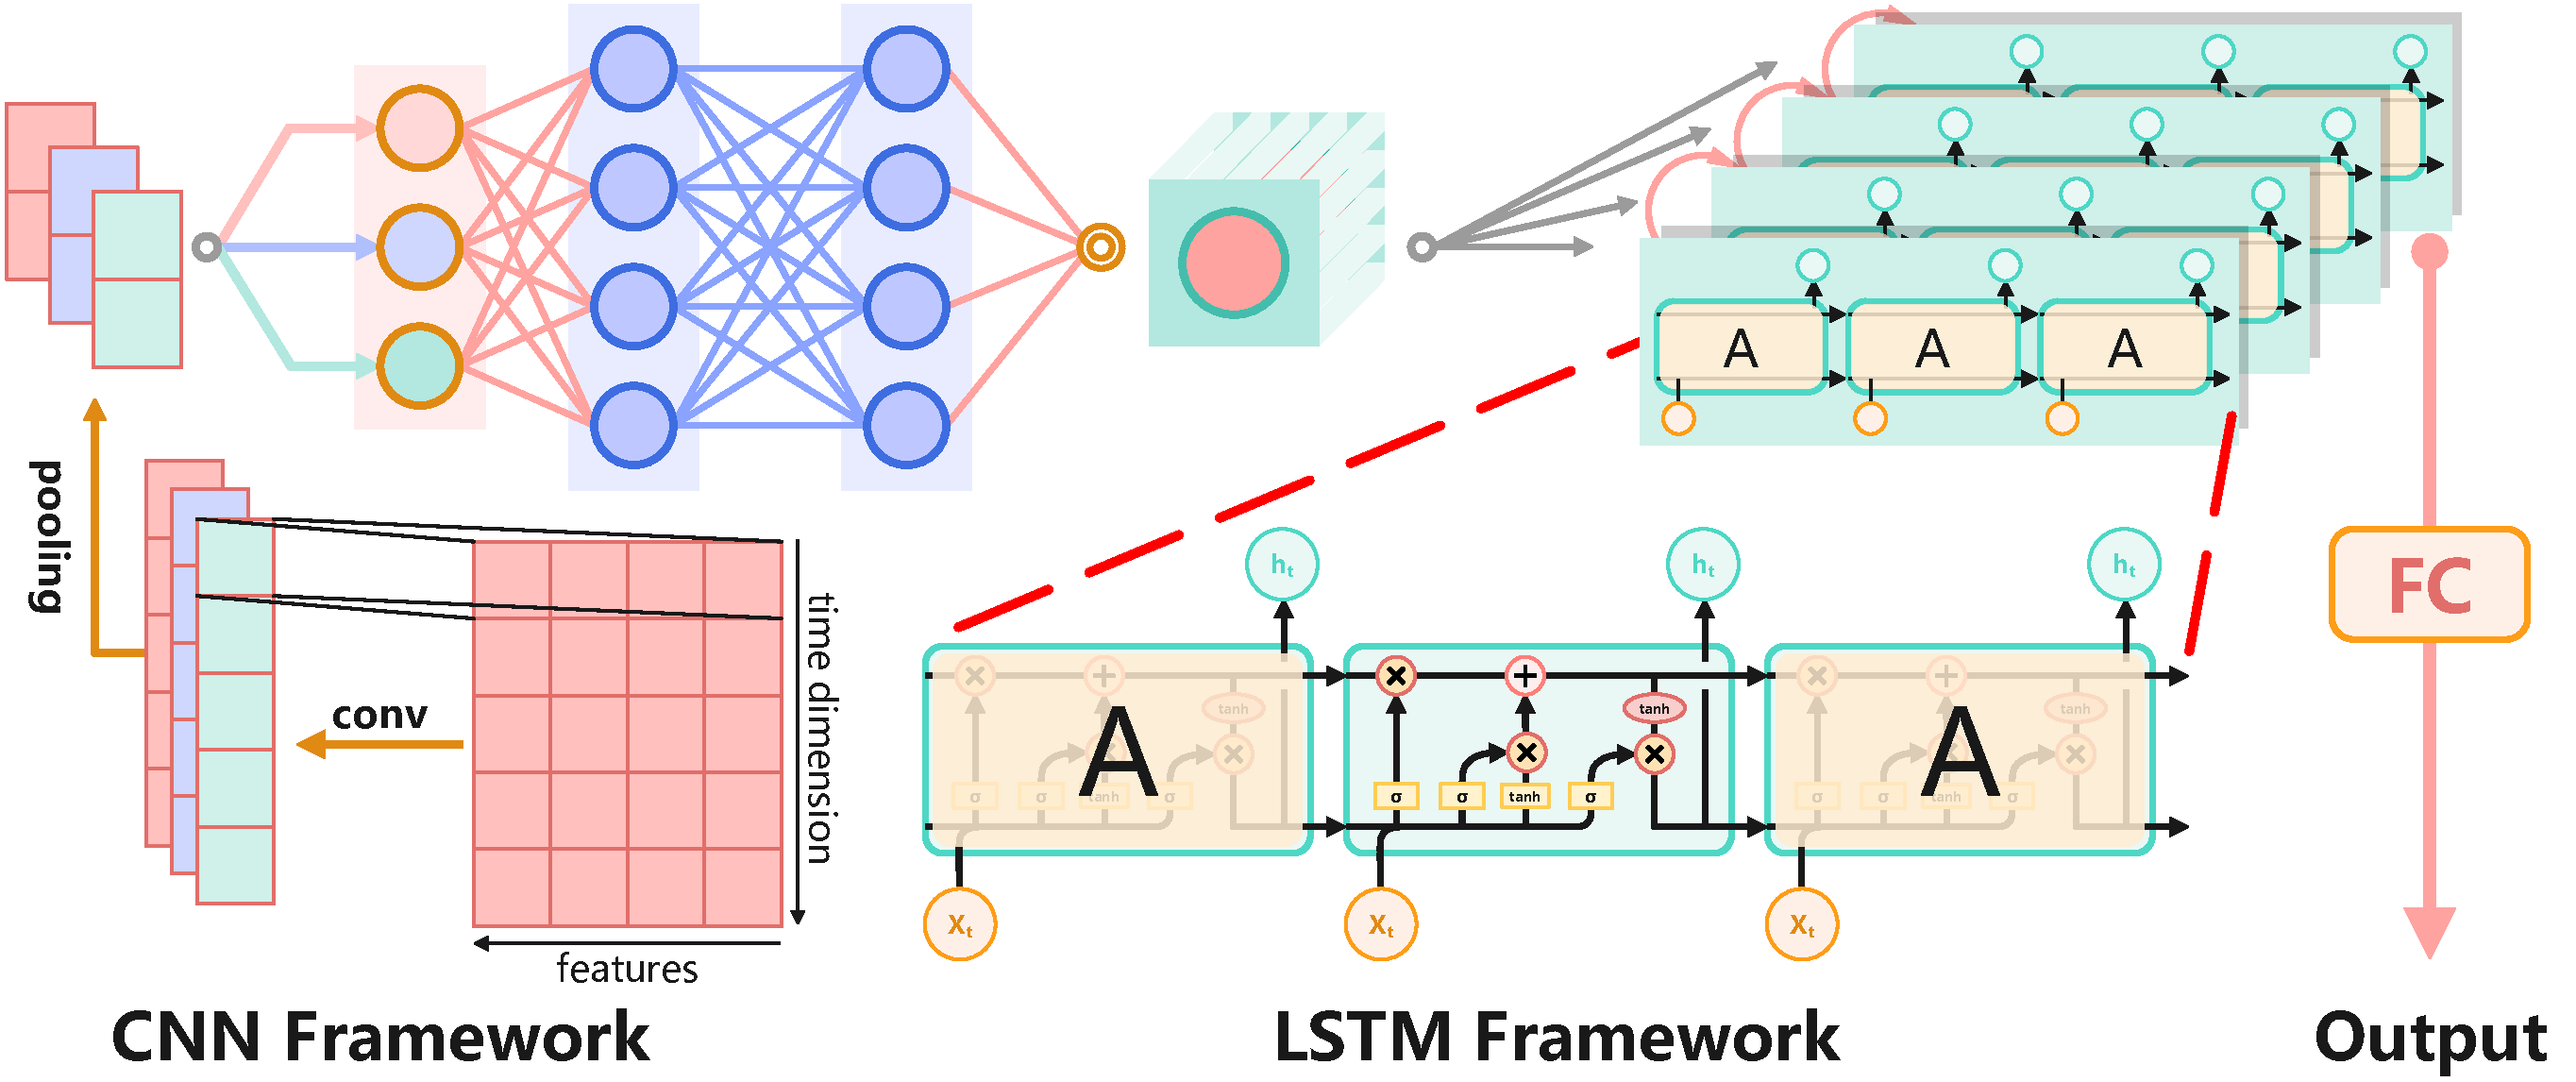
\includegraphics[width=1.0\textwidth]{./Img/CNN_LSTM结构图.pdf}
  \caption{CNN-LSTM整体结构图}\label{fig:4-11}
\end{figure}

当前气象研究领域的先进方法当中,目前较为流行的方法是融合了卷积神经网络(CNN)与长短时记忆网络(LSTM)的混合模型 \cite{HJKZ2024011600J}\cite{JYGC20240415002},大量的实验结果表明这种混合模型可以显著提高预测的准确性。受CNN-LSTM混合模型思想的启发,我们在LSTM模型的基础之上,引入了CNN网络,旨在于把时间序列数据转换成图像并使用深度学习技术来提取特征能够有效捕捉气象数据中的时间序列非线性变化,CNN与LSTM结合之后实际的架构设计如图 \ref{fig:4-11} 所示。





\begin{figure}[h]
  \centering
  \begin{subfigure}{0.48\textwidth}
      \centering
      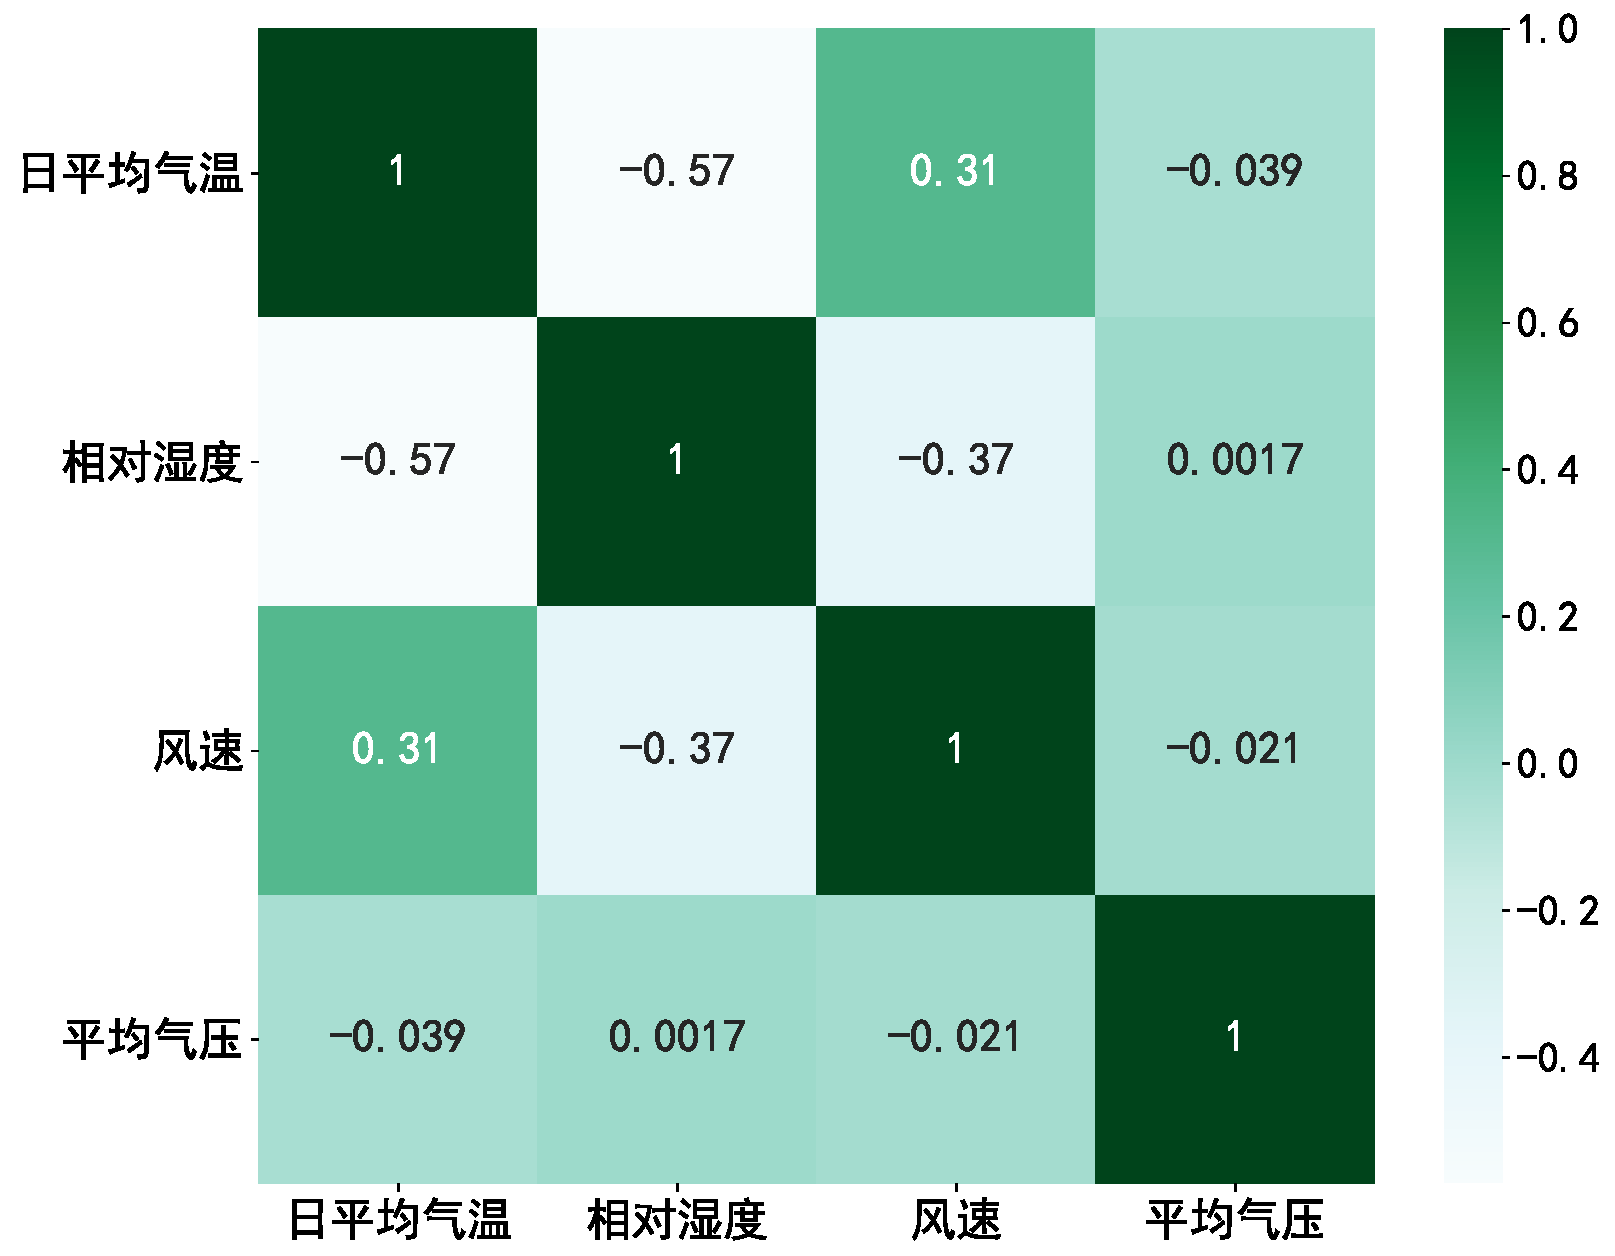
\includegraphics[width=\linewidth]{./Img/CNN-LSTM相关性热力图.pdf}
      \caption{有效数据中四项指标的相关性热力图}\label{fig:4-13-b}
  \end{subfigure}
  \hfil
  \begin{subfigure}{0.48\textwidth}
      \centering
      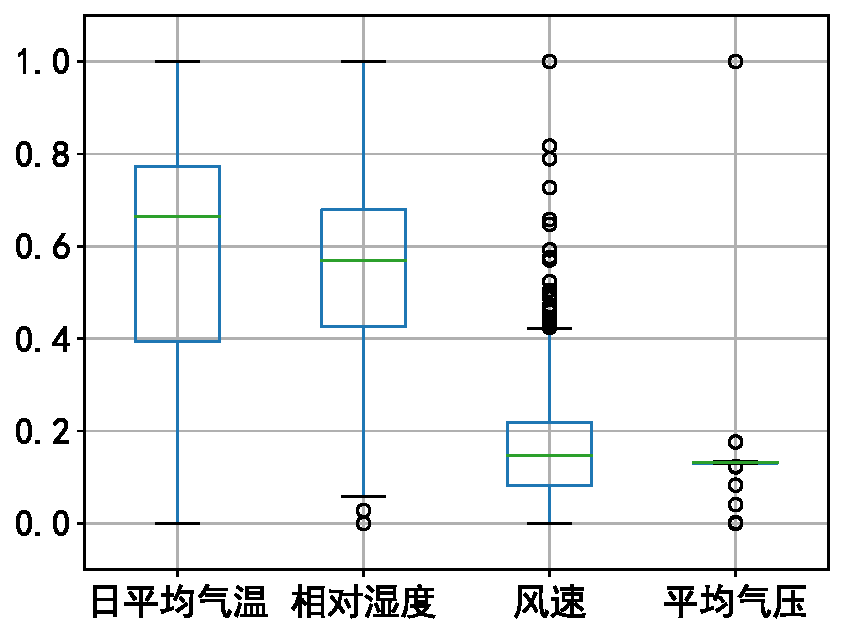
\includegraphics[width=\linewidth]{./Img/CNN-LSTM相关性箱线图.pdf}
      \caption{有效数据中四项指标的箱型图}\label{fig:4-13-c}
  \end{subfigure}
  \caption{四项指标的相关性热力图与箱型图}
  \label{fig:4-17-b}
\end{figure}




对于新的CNN-LSTM框架,为了更好的评估新框架的预测性能,我们严谨选择了新的一组气象数据作为数据集,新的数据集涵盖了2013年1月至2017年4月这段时间日平均气温、相对湿度、风速以及平均气压等指标的气象数据,为了深入探讨特征随机性对模型泛化能力的影响,我们采用了相关性热力图和箱型图这两种可视化工具,如图 \ref{fig:4-13-b} 和 \ref{fig:4-13-c} 所示,以便直观地揭示了不同指标之间的相关性和随机波动关系。

\begin{table}[h]
    \caption{2013年1月-2017年4月期间的有效气象数据}\label{tab:CNN_LSTM_data}
    \centering
    \resizebox{0.8\linewidth}{!}
    {\begin{tabular}{*5{c}}\toprule
        时间 & 日平均气温(${}^{\circ}\text{C}$) & 相对湿度($\%RH$) & 风速($m/s$)  & 平均气压($P_a$) \\ 
        \midrule
        2013-01-01 & 10.0 & 84.5 & 0.0 & 1015.67 \\
        2013-01-02 & 7.4 & 92.0 & 2.98 & 1017.8 \\
        2013-01-03 & 7.17 & 87.0 & 4.63 & 1018.67 \\
        2013-01-04 & 8.67 & 71.33 & 1.23 & 1017.17 \\
        2013-01-05 & 6.0 & 86.83 & 3.70 & 1016.5 \\
        2013-01-06 & 7.0 & 82.8 & 1.48 & 1018.0 \\
        2013-01-07 & 7.0 & 78.6 & 6.30 & 1020.0 \\
        2013-01-08 & 8.86 & 63.71 & 7.14 & 1018.71 \\
        $\cdots$ & $\cdots$ & $\cdots$ & $\cdots$ & $\cdots$ \\
        2017-04-18 & 34.0 & 27.33 & 7.81 & 1003.11 \\
        2017-04-19 & 33.5 & 24.13 & 9.03 & 1000.88 \\
        2017-04-20 & 34.5 & 27.50 & 5.56 & 998.63 \\
        2017-04-21 & 34.25 & 39.38 & 6.96 & 999.88 \\
        2017-04-22 & 32.90 & 40.90 & 8.90 & 1001.60 \\
        2017-04-23 & 32.88 & 27.50 & 9.96 & 1002.13 \\
        2017-04-24 & 32.00 & 27.14 & 12.16 & 1004.14 \\
        \bottomrule
    \end{tabular}}
\end{table}

在相关性热力图 \ref{fig:4-13-b} 中,我们可以观察到日平均气温与相对湿度之间存在中等到较强的负相关性(-0.57),而与风速之间则有轻微的正相关性(0.31),与气压的相关性则几乎可以忽略不计。此外,风速和相对湿度之间的相关性为中等程度的负相关(-0.37)。在箱型图 \ref{fig:4-13-c} 中,日平均气温和相对湿度的分布较为集中,且大部分数据位于中间位置,说明这两个变量的取值相对稳定。风速的分布则呈现出较大的差异,数据分散在较宽的范围内,说明风速的变化较大。平均气压的分布也轻度分散,整体上取值较低,说明平均气压的值相对较小。总体来看,这四个指标之间展现出了复杂而多样的相关性模式,既有正相关也存在负相关,这不仅丰富了模型对这些指标相互依赖关系和潜在影响的理解,而且有助于提升模型的泛化性能。通过这种方式,我们确保了模型在面对未知数据集时,能够保持广泛的适用性和高度的可靠性。


在模型训练之前,我们首先对数据进行了预处理。同样遵循LSTM模型的数据预处理规范,我们对数据集中出现的缺失值和异常值采取了均值填补策略,剔除了缺失超过三项气象指标的数据记录。经过数据处理步骤后,我们得到了1462条气象观测数据。这些数据包括了2013年至2017年的日平均气温。我们将整理后的数据部分以表格形式展示,如表 \ref{tab:CNN_LSTM_data} 所示。此外,我们还进行了数据可视化处理,可视化后日平均气温数据如图 \ref{fig:4-13-a} 所示。



\begin{figure}[h]
  \centering
  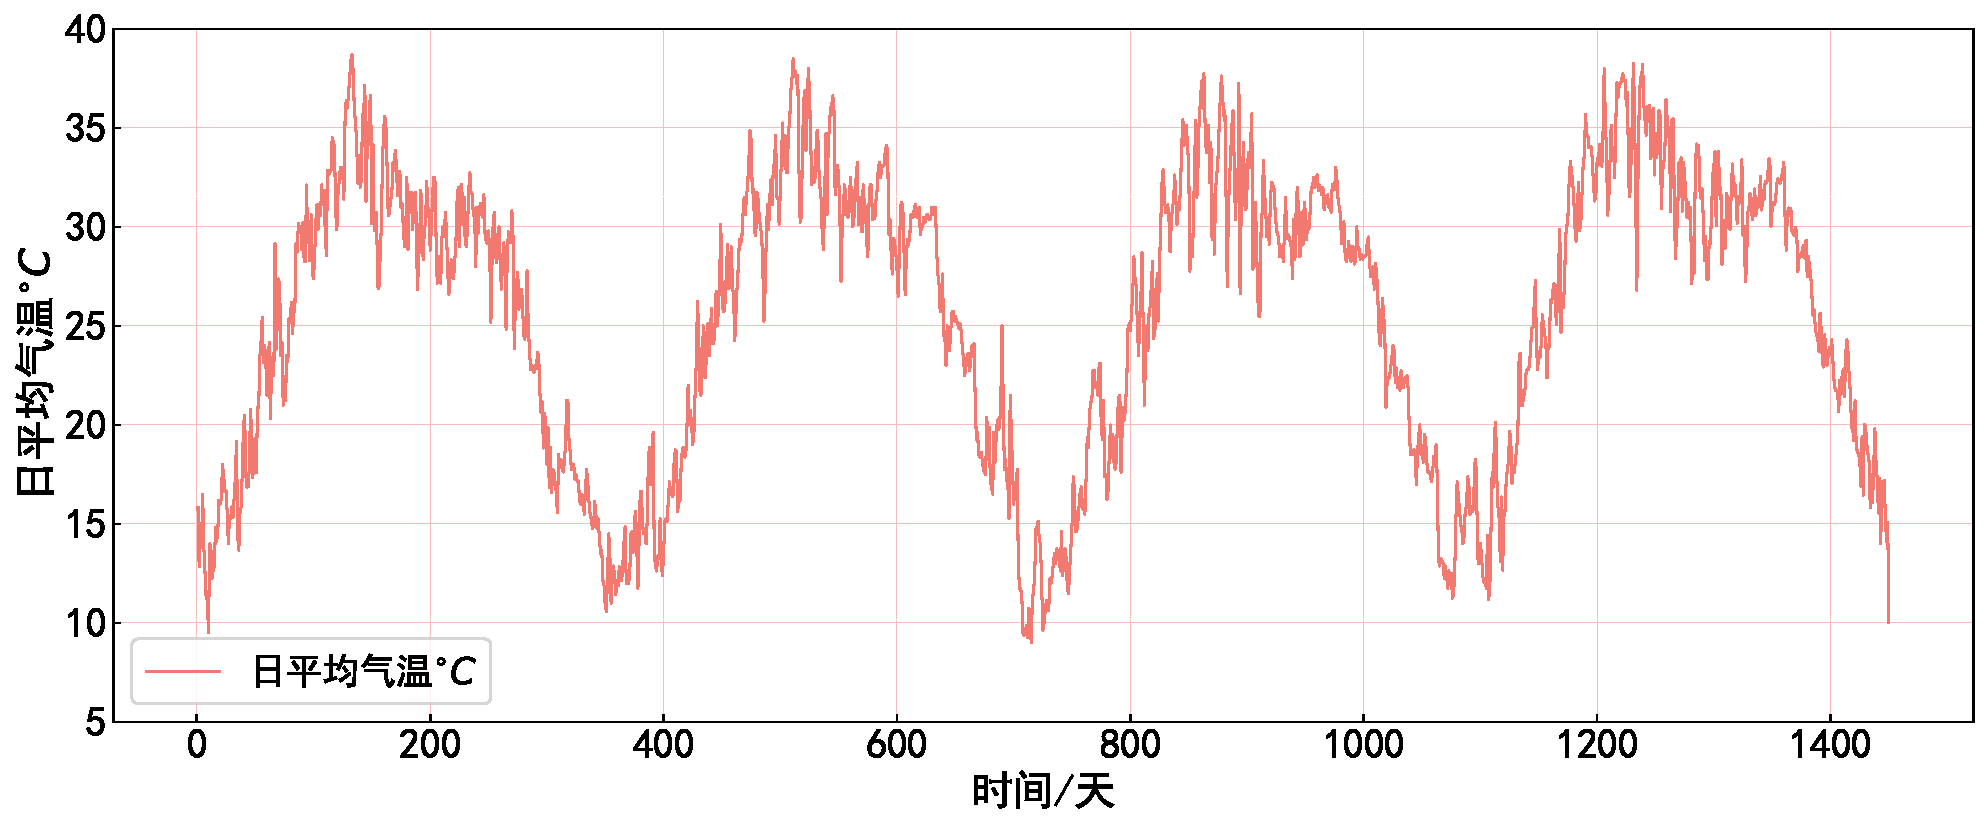
\includegraphics[width=1.0\textwidth]{./Img/CNN_LSTM_origin_data.pdf}
  \caption{2013年-2017年日平均气温}\label{fig:4-13-a}
\end{figure}


\begin{figure}[h]
  \centering
  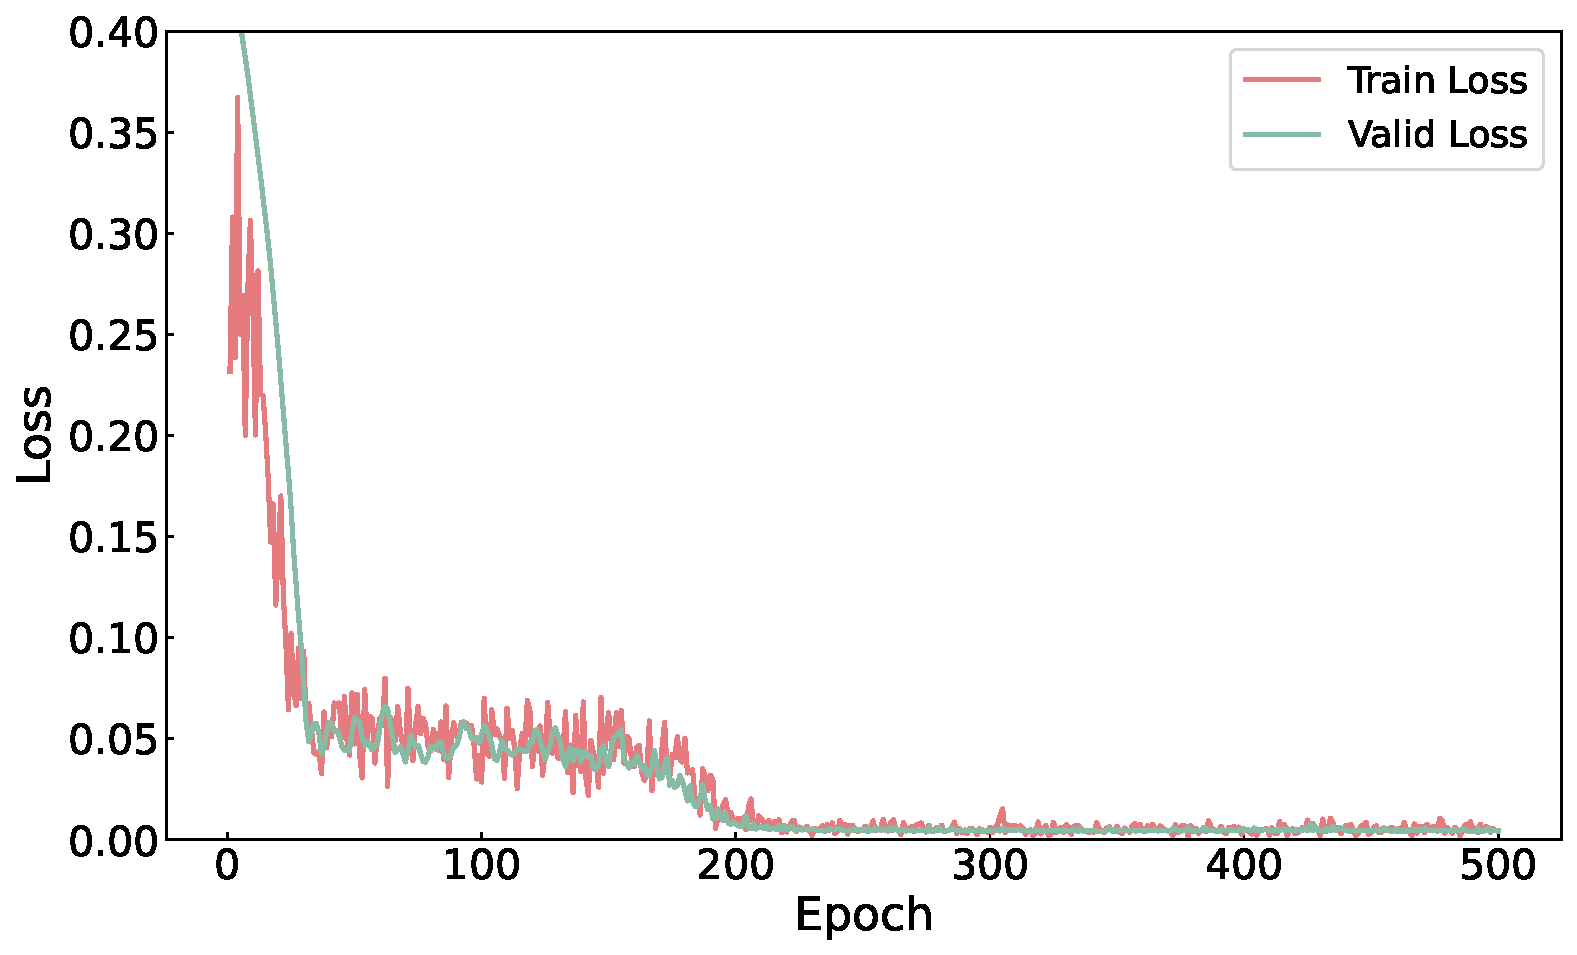
\includegraphics[width=0.7\textwidth]{./Img/CNN_LSTM_loss.pdf}
  \caption{CNN-LSTM模型的训练损失与验证损失}\label{fig:4-12}
\end{figure}



\begin{figure}[t]
  \centering
  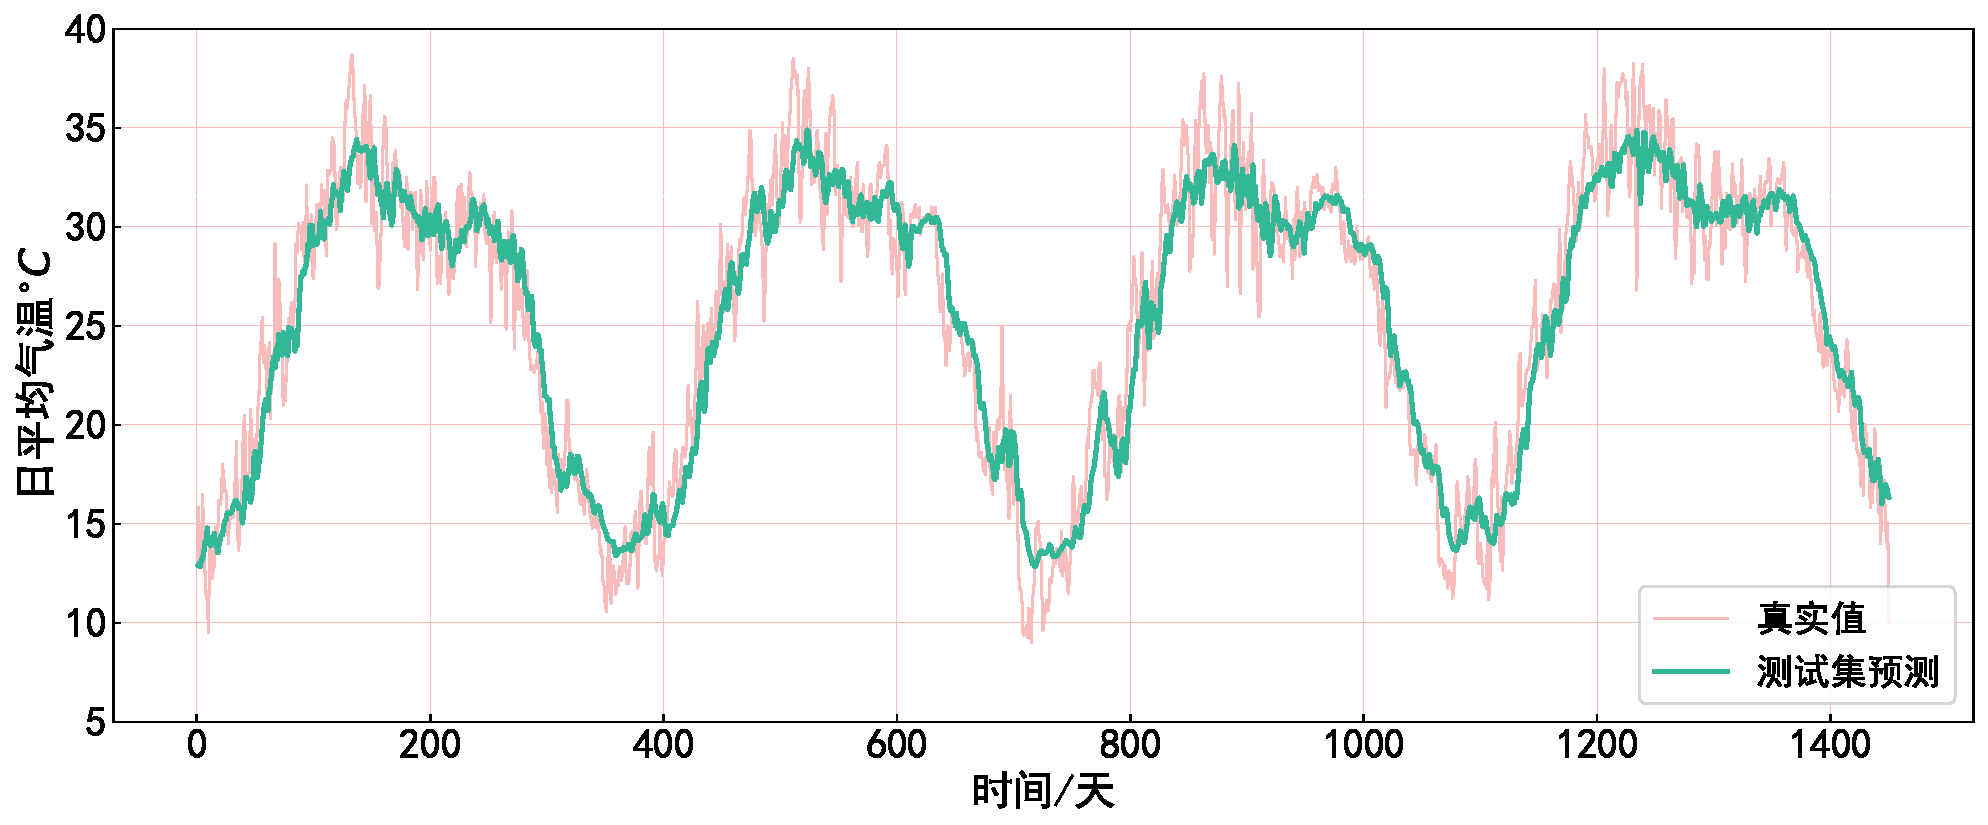
\includegraphics[width=1.0\textwidth]{./Img/CNN_LSTM_test_pre.pdf}
  \caption{CNN-LSTM模型针对2013-2017年日平均气温的预测结果}\label{fig:4-13}
\end{figure}


接下来,我们进入模型训练阶段,首先对所有数据执行了归一化处理,并选择了日平均气温作为关键的评价指标,设定的训练次数Epoch为500次,训练时的每一批量大小为16,采用ReLU和Adam分别作为激活函数和优化器。随后,将这些配置应用于CNN-LSTM模型中展开训练,模型训练过程的训练损失和验证损失如图 \ref{fig:4-12} 所示。在训练完成之后,进入模型推理阶段,使用训练好的模型针对指定时间段 [1,1462] 这个时间区间进行预测,得到的预测结果如图 \ref{fig:4-13} 所示,经过计算,得到预测值和真实值的均方误差为:$5.0165 {}^{\circ}\text{C}{}^2$。

\begin{figure}[h]
  \centering
  \begin{subfigure}{0.48\textwidth}
    \centering
    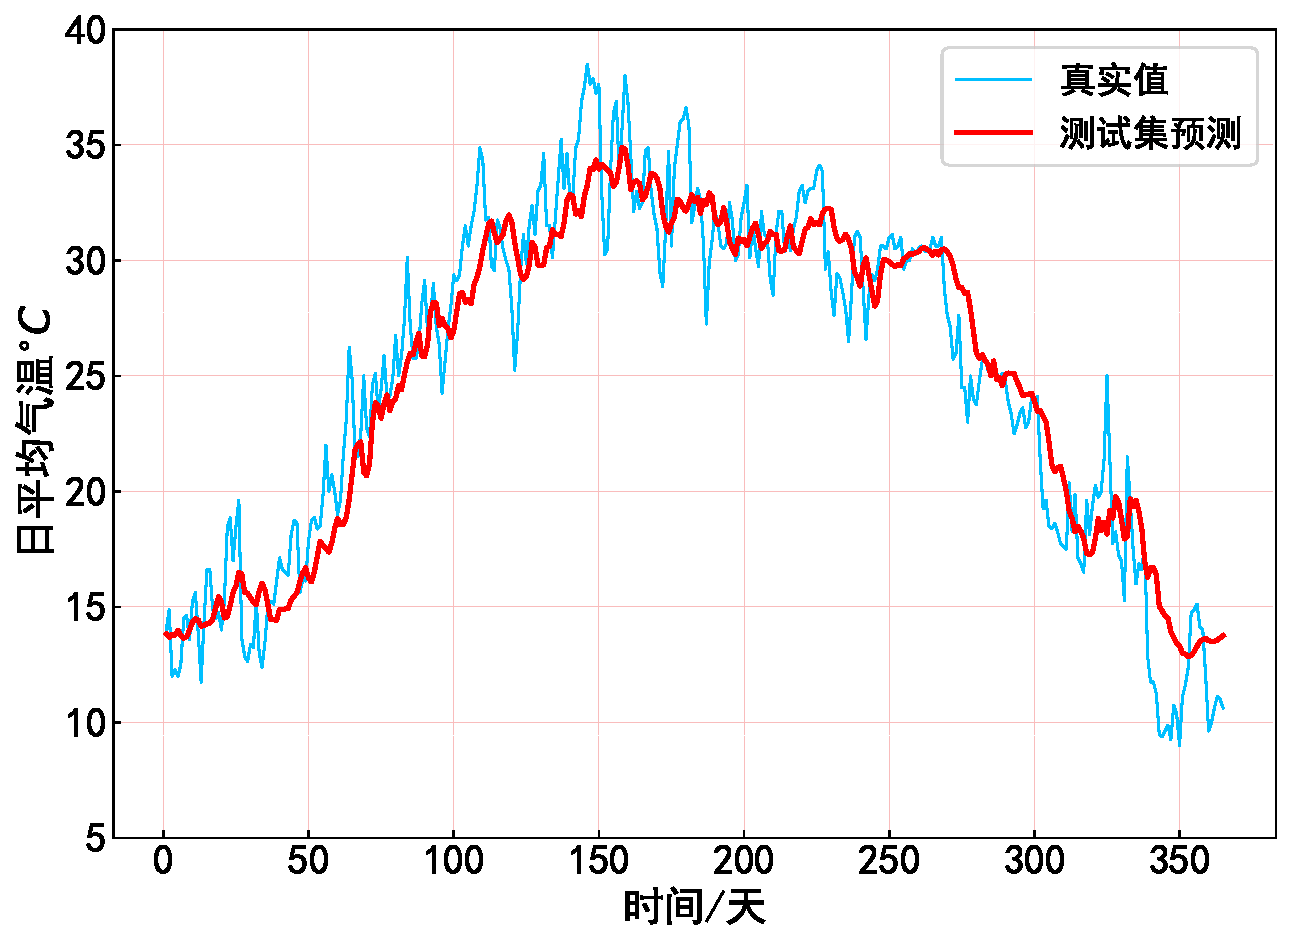
\includegraphics[width=\linewidth]{./Img/CNN_LSTM_test_first_pre.pdf}
    \caption{2014年全年日平均气温预测值与真实值对比}\label{fig:4-14}
  \end{subfigure}
  \hfil
  \begin{subfigure}{0.48\textwidth}
    \centering
    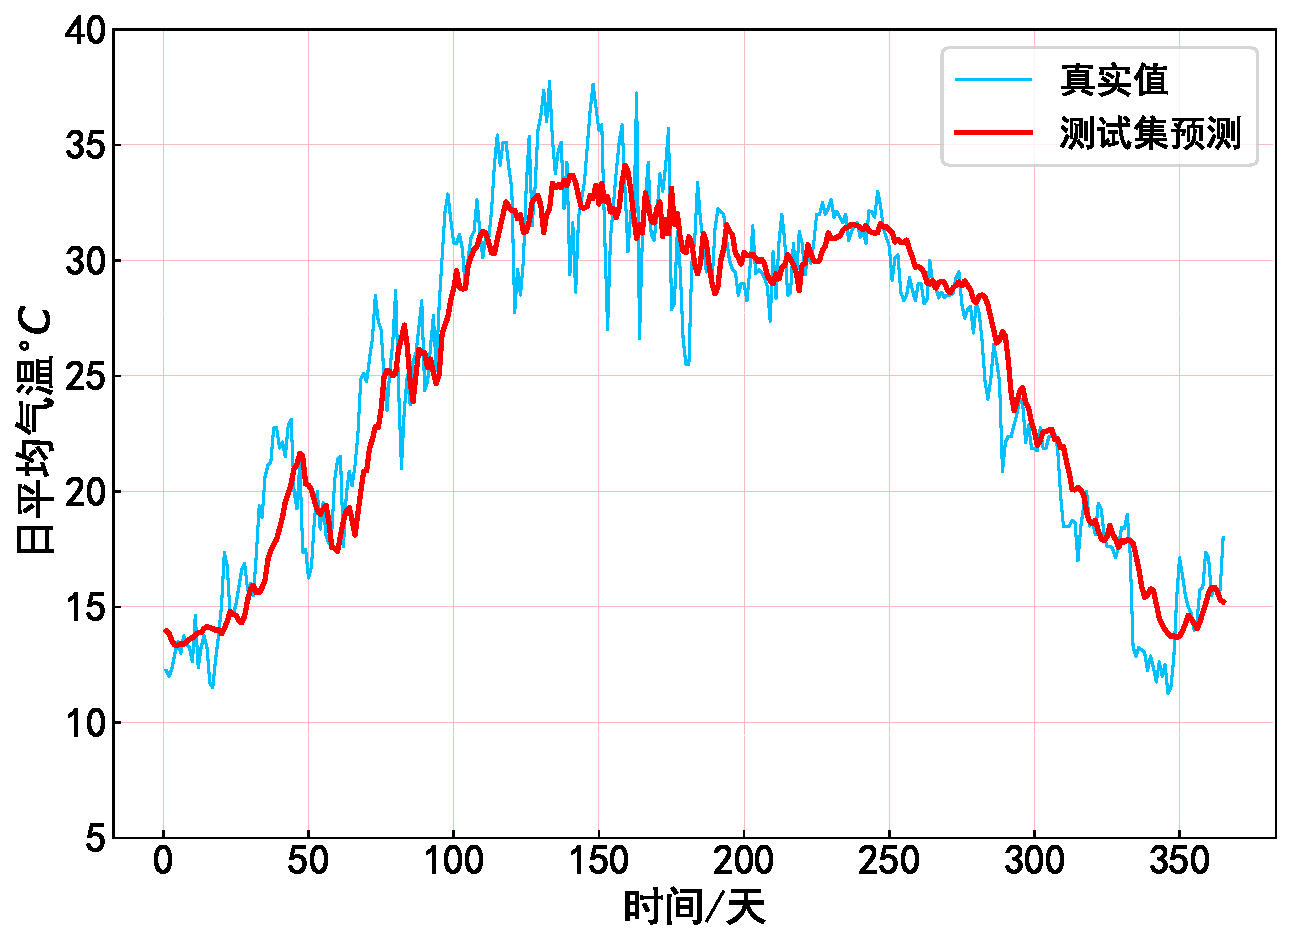
\includegraphics[width=\linewidth]{./Img/CNN_LSTM_test_section_pre.pdf}
    \caption{2015年全年日平均气温预测与真实值对比}\label{fig:4-15}
  \end{subfigure}
  \caption{2014年与2015全年日平均气温预测结果}
  \label{fig:4-17-all}
\end{figure}

在分析图 \ref{fig:4-13} 中的气象数据预测时,我们可以看到预测值与真实值整体上保持了较好的一致性,尤其是在日平均气温的预测中,模型能够较为准确地捕捉到温度的变化趋势。然而,在一些特定的时间段,如风速和平均气压的波动较大时,预测值与真实值之间存在一定的偏差。这可能意味着模型在这些情况下对风速和气压的处理不够精确,或者是模型过于专注于日平均气温的预测,而忽视了其他因素的综合影响。为了更清晰地显示真实值与预测值的差别,我们分别挑选出了2014年和2015年的全年日平均气温真实值和预测值进行可视化,如图 \ref{fig:4-17-all} 中的图 \ref{fig:4-14} 和图 \ref{fig:4-15} 所示。


此外,综合分析图 \ref{fig:4-8}、图 \ref{fig:4-9}、图 \ref{fig:4-10}、图 \ref{fig:4-13}、图 \ref{fig:4-14} 以及图 \ref{fig:4-15},单独的LSTM模型在小规模多个指标的数据集上表现出色,其预测结果与真实值的高度一致性和拟合程度不仅彰显了模型的强大泛化能力,也充分验证了我们在特征工程、模型架构设计以及超参数调优策略方面的有效性和准确性。然而,对于新型的CNN-LSTM架构,它在相对大型且少量指标的数据集上,尤其是在波动程度较大的数据,如极端天气事件前后,预测误差较大。这可能是因为模型未能充分学习到这些特殊情况下的特征,或者在处理异常数据时的鲁棒性不足。因此,为了提高预测精度,我们可以考虑对模型进行改进,例如引入更多的特征变量、优化模型结构或调整参数等。虽然当前的预测模型在一定程度上能够反映日平均气温的变化趋势,但在处理极端天气和其他影响因素时仍存在一些不足之处。未来的研究可以进一步探讨如何提高模型的预测能力,以更好地支持气象数据的分析和预报工作。



\subsection{LGESD细粒度哈希图像检索模型}

\subsubsection{模型介绍}

\begin{figure}[h]
  \centering
  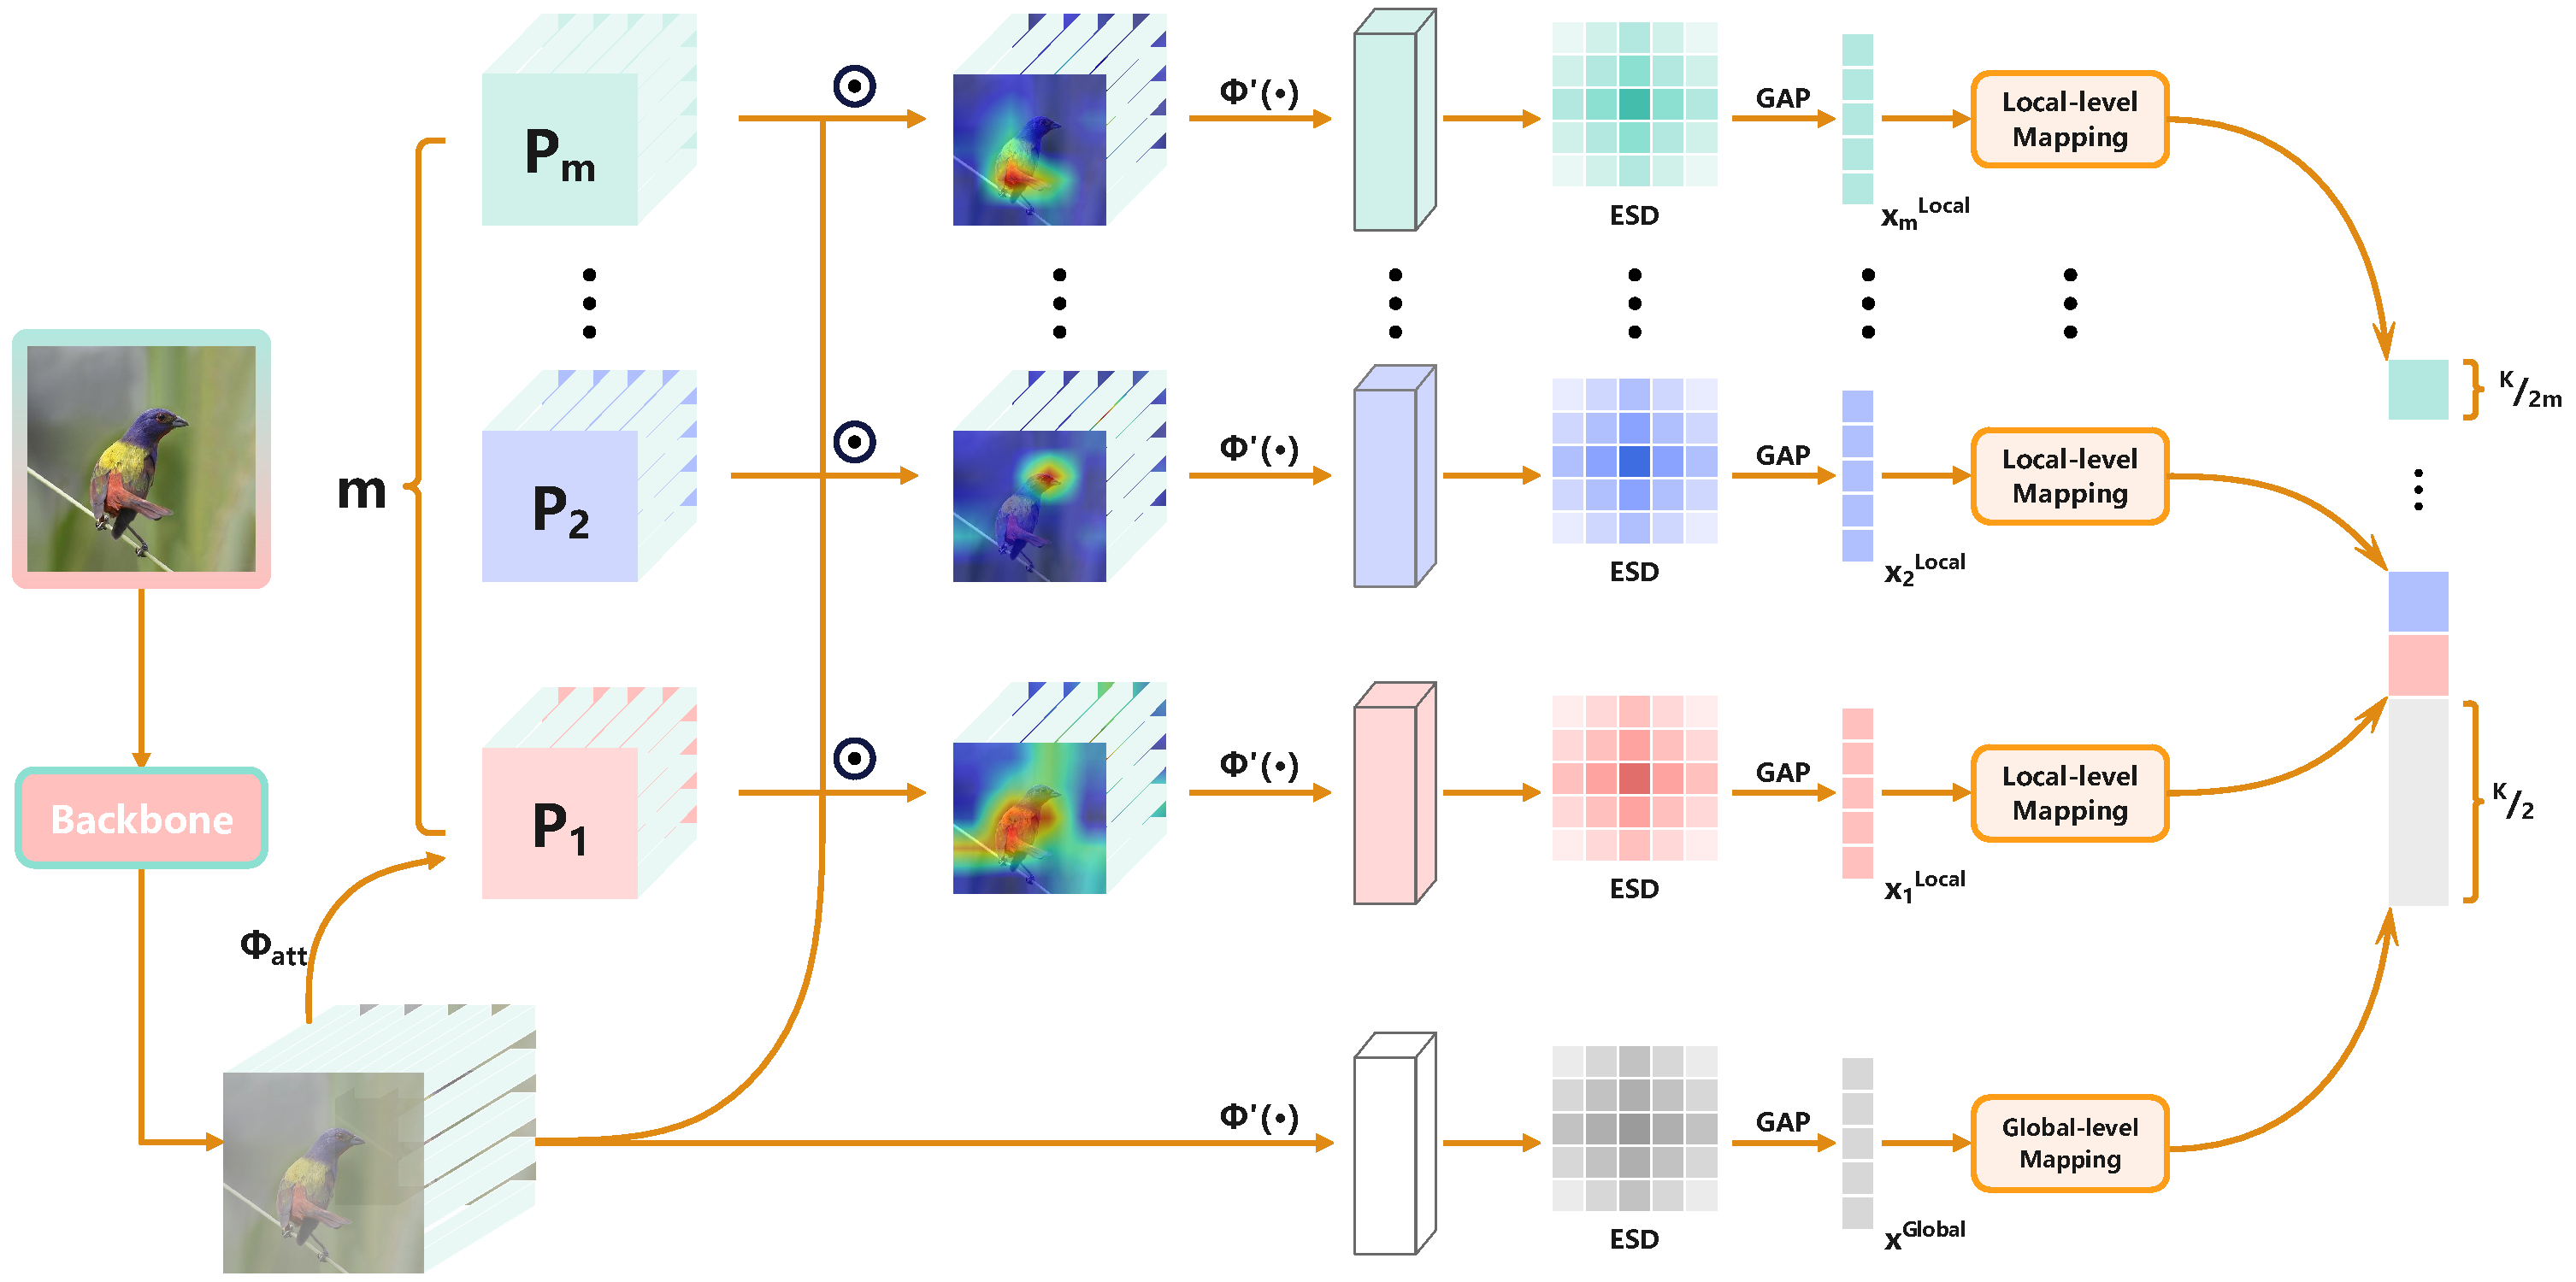
\includegraphics[width=1.0\textwidth]{./Img/完整架构图.pdf}
  \caption{LGESD整体架构图}\label{fig:4-21}
\end{figure}

通常情况下,在细粒度视觉识别任务中,兼顾对象的整体(全局)特征与局部细节(部分级)特征被认为是极为关键的 \cite{wei2021finegrained}。基于这一认识,我们提出了 \textbf{LGESD} 框架,一个基于显式空间衰减的局部与全局学习(\textbf{L}ocal and \textbf{G}lobal learning of \textbf{E}xplicit \textbf{S}patial \textbf{D}ecay)的细粒度哈希检索框架,我们在该框架中构建了一个双轨结构:一方面是一个专注于全局特征提取的学习分支,另一方面则是专攻局部模式学习的分支,架构详情如图 \ref{fig:4-21} 所示。在双轨结构设计的基础上,哈希码生成机制同样采用了双层设计,包含一个全局哈希映射单元和一个局部哈希映射单元。

其中,全局哈希映射单元旨在提炼反映对象整体信息的二进制码;而局部哈希映射单元则进一步细分,通过 $m$ 个子线性编码器模块来实现,专门用于明确提取每个组成部分的局部二进制哈希码,以此增强对细微特征的区分能力。因此,所得的哈希码内嵌了物体的全局身份信息与局部结构特征。此外,我们在该框架中创新性的引入了一种基于显式超先验的空间衰减注意机制(\textbf{E}xplicit \textbf{S}patial \textbf{D}ecay,\textbf{ESD}),该机制在下游处理阶段发挥着核心作用,确保生成的全局特征与对应局部特征既能互补又能凸显各自的独特性,从而提升特征表达的辨别力。

\subsubsection{整体框架设计}

对于输入的每一张图像 $\mathrm{I}$,经过一个卷积神经网络 $\Phi_{\mathrm{CNN}}(\cdot)$ 提取出它的深度激活张量 $\mathrm{T}$:
\begin{equation}
    \mathrm{T}=\Phi_{\mathrm{CNN}}(\mathrm{I})\in\mathbb{R}^{C\times H\times W}
\end{equation}

基于深度激活张量 $\mathrm{T}$,在全局特征学习分支中执行配备一叠卷积层的全局级转换网络 $\phi(\cdot)$,如下所示:
\begin{equation}
\hat{\mathrm{T}}=\phi(\mathrm{T};\theta_{\mathrm{global}})\in\mathbb{R}^{C^{\prime}\times H^{\prime}\times W^{\prime}}
\end{equation}

其中 $\theta_{\mathrm{global}}$ 表示 $\phi(\cdot)$的参数配置,而在局部特征学习当中,分别划分了 $m$ 个学习阶段,并为每一个学习阶段的添加了一个注意力引导机制 $\mathrm{P}_i = \phi_{\mathrm{att}}(T;\theta_{\mathrm{att}}), \mathrm{P}_i \in \mathrm{R}^{\frac{C}{m} \times H \times W}$,用于在每个阶段学习生成注意力图 $M_i$,在得到每个学习阶段注意力图之后,通过逐个元素点乘的方式评估 $H \times W$ 个元素当中被关注的深度描述符。
\begin{equation}
    \mathrm{T}_i^{\prime}=M_i\odot \mathrm{T}, \quad i \in \{1,2,\cdots,m \}
    \label{eq:eq_4_m}
\end{equation}

获得深度描述符之后,为了获得特定于语义的表示,我们选择使用与 $\phi(\cdot)$ 具有相同结构的局部级变换网络 $\phi^{\prime}(\cdot)$ 将 $\mathrm{T}_i^{\prime}$ 转换为 $\hat{\mathrm{T}}_i^{\prime}$:
\begin{equation}
    \hat{\mathrm{T}}_i^{\prime}=\phi^{\prime}(\mathrm{T}_i^{\prime};\theta_{\mathrm{local}})\in\mathbb{R}^{C^{\prime}\times H^{\prime}\times W^{\prime}}
\end{equation}

其中 $\theta_{\mathrm{local}}$ 表示 $\phi^{\prime}$ 的参数配置。最后,通过对 $\hat{\mathrm{T}}$ 和 $\hat{\mathrm{T}}_i^{\prime}$ 执行全局平均池化(Global Average Pooling,GAP),可获得对象级特征 $x^{global}$ 和 $m$ 个部分级特征 $x^{local}_i$。为了生成类似二进制的代码,我们采用了一个由 $m + 1$ 个线性编码器范式组成的二进制代码映射模块 $\mathrm{W}=\{\mathrm{W}^{global};\mathrm{W}_1^{local};\mathrm{W}_2^{local};\ldots;\mathrm{W}_m^{local}\}$ 将 $x^{global}$ 和 $x_i^{local}$ 分别映射为 $\mathrm{v}^{global}$ 和 $\mathrm{v}_i^{local}$。最后,再次使用哈希学习模块将 $\mathrm{v}^{global}$ 和 $\mathrm{v}_i^{local}$ 转为最终的二进制哈希码 $\mathrm{u}=[\mathrm{u}^{global};\mathrm{u}_1^{local};\mathrm{u}_2^{local};\cdots;\mathrm{u}_m^{local}]$。

\subsubsection{基于显式超先验的空间衰减注意机制}

RetNet \cite{sun2023retentive} 在大语言模型任务当中首次在注意力中使用时间衰减这个概念,并在实际的实验过程中取得了极其优秀的性能。在初步处理方式上,采用RetNet的思想,对于给定的一个输入序列 $x=x_{1}\cdots x_{|x|}$,通过自回归的方式将其编码为 $X^0 = [\mathrm{x}_1,\cdots,\mathrm{x}_{|x|}] \in \mathbb{R}^{|x|\times d_{\mathrm{model}}}$,其中 $d_{\mathrm{model}}$ 表示隐含层的维度, 然后计算上下文向量表示 $X^l=\mathrm{RetNet}_l(X^{l-1}),l\in[1,L]$。

\begin{figure}[h]
    \centering
    \begin{subfigure}[b]{0.23\textwidth}
        \centering
        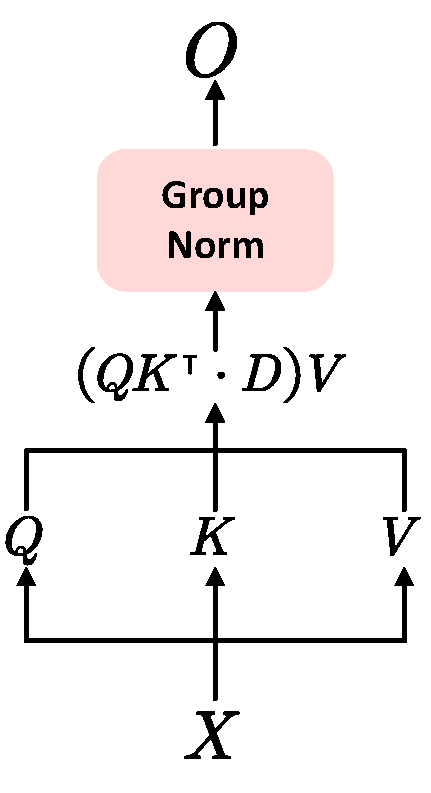
\includegraphics[width=\linewidth]{Img/并行计算过程.pdf}
        \caption{并行计算过程}
        \label{fig:4-3_a}
    \end{subfigure}
    \begin{subfigure}[b]{0.58\textwidth}
        \centering
        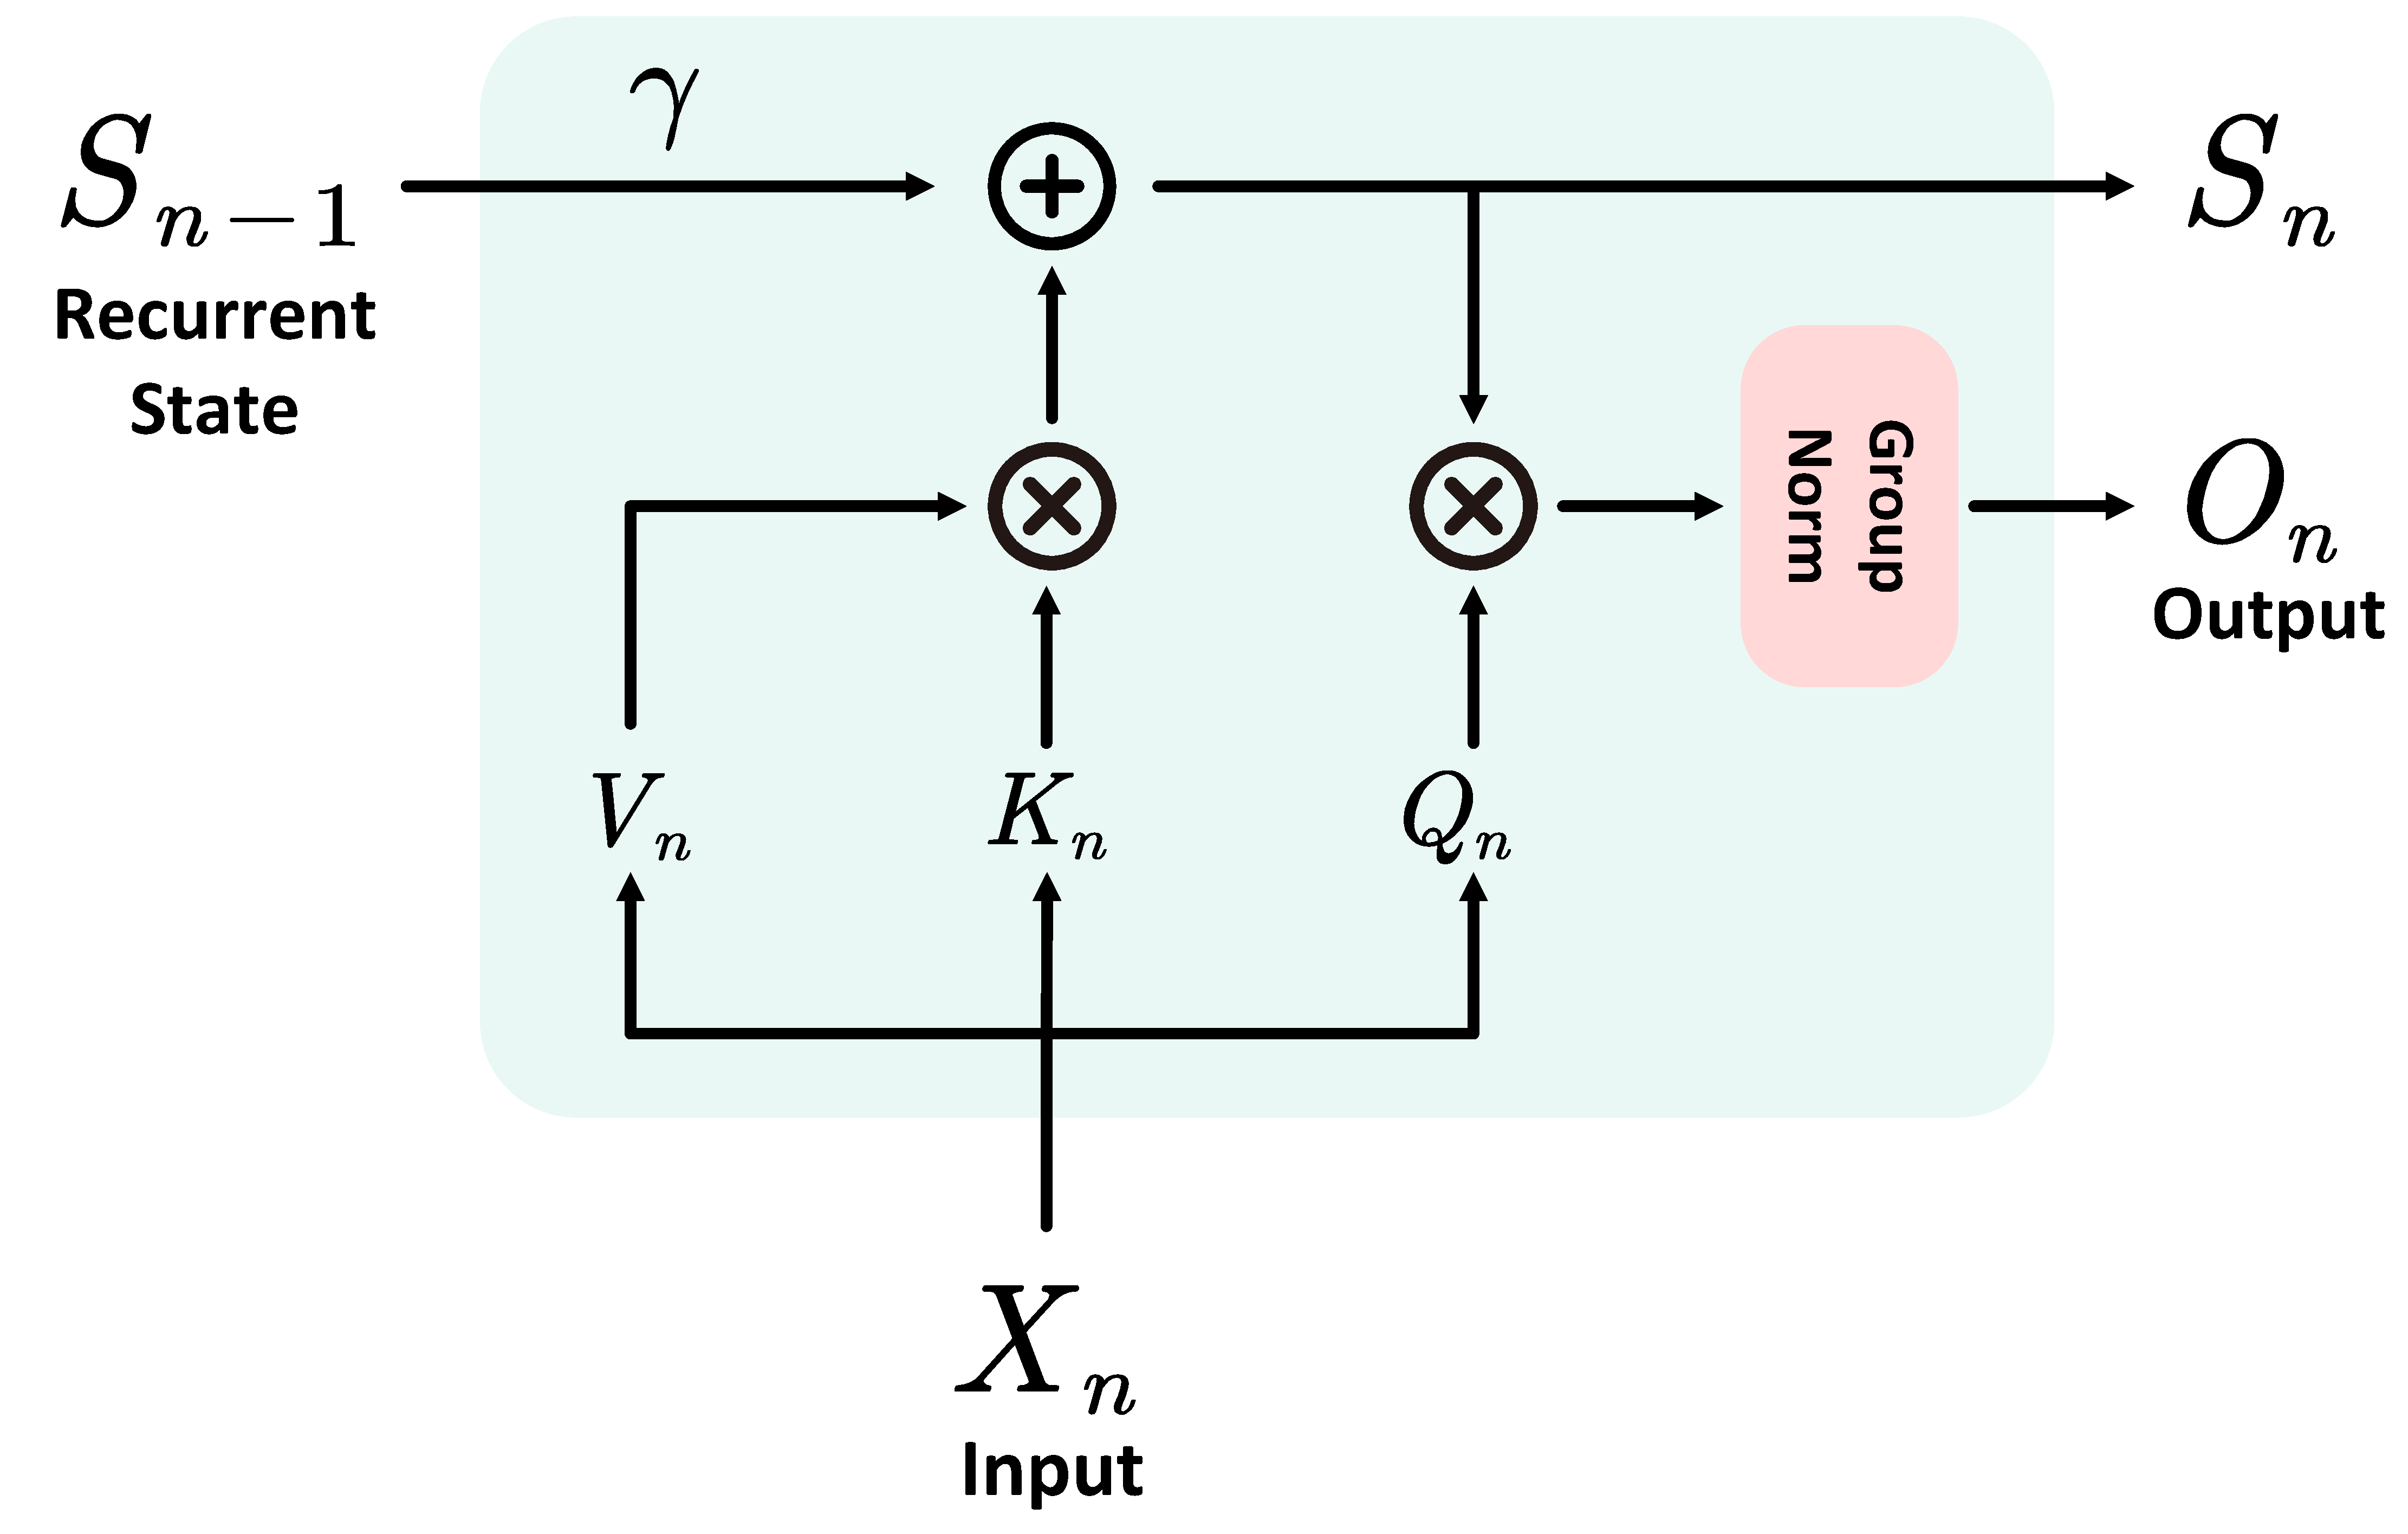
\includegraphics[width=\linewidth]{Img/循环计算过程.pdf}
        \caption{循环计算过程}
        \label{fig:4-3_b}
    \end{subfigure}
    \caption{RetNet的循环化和并行化双重计算过程}\label{fig:4-3}
\end{figure}


经过处理得到的 $X\in\mathbb{R}^{|x|\times d_{\mathrm{model}}}$,我们将其投影到一维的函数 $v(n)=X_n\cdot  {w}_V$,在此过程中,RetNet 设计了一个循环化和并行双重计算过程,如图 \ref{fig:4-3} 所示,使得 $v(n)$ 经过中间状态 $s_n$ 得到输出 $o(n)$,具体的循环计算公式如下:
\begin{align}
    s_n &=As_{n-1}+K_n^\intercal v_n, \quad A\in\mathbb R^{d\times d},K_n\in\mathbb R^{1\times d} \label{eq:4-0}\\
    o_n &=Q_ns_n=\sum_{m=1}^nQ_nA^{n-m}K_m^\intercal v_m, \quad Q_n\in\mathbb R^{1\times d} \label{eq:4-1}
\end{align}

其中的 $v_n$ 和 $o_n$ 即为 $v(n)$ 和 $s(n)$,之后,定义一个可学习的矩阵:$W_Q,W_K\in\mathbb{R}^{d\times d}$,因此,投影 $Q_n$ 和 $K_n$的内容感知如下:
\begin{align}
    Q=XW_Q,\quad K=XW_K
\end{align}

然后对公式 \ref{eq:4-0} 中的 $A$ 矩阵进行奇异值分解操作,得到 $A = \Lambda(\gamma e^{i\theta})\Lambda^{-1}, \gamma,\theta\in\mathbb{R}^d$,同理,对于 $n-m$ 次循环,可以得到 $A^{n-m} = \Lambda(\gamma e^{i\theta})^{n-m}\Lambda^{-1}, \gamma,\theta\in\mathbb{R}^d$,用这个 $A^{n-m}$ 的表达式替换掉公式 \ref{eq:4-1} 中的 $A^{n-m}$,整理后的 $o_n$ 的计算公式如下:
\begin{equation}
  \begin{split}
    o_{n}& =\sum_{m=1}^nQ_n(\gamma e^{i\theta})^{n-m}K_m^\intercal v_m \\
    &=\sum_{m=1}^n(Q_n(\gamma e^{i\theta})^n)(K_m(\gamma e^{i\theta})^{-m})^\intercal v_m \\
    &=\sum_{m=1}^n\gamma^{n-m}(Q_ne^{in\theta})(K_me^{im\theta})^\dagger v_m
  \end{split}
\end{equation}

其中 $\dagger$ 表示共轭转置,之后针对整体的计算过程进行并行化,如图 \ref{fig:4-3_a} 所示,具体的表达式如下所示:
\begin{align}
    Q=(XW_Q)\odot\Theta,\quad K &=(XW_K)\odot\overline{\Theta},\quad V=XW_V\\
    \Theta_n= e^{in\theta},\quad D_{nm}&=\begin{cases}\gamma^{n-m},&n\geq m\\0,&n<m\end{cases}\\
    \text{Retention}(X) &=(QK^\intercal\odot D)V
\end{align}

\begin{figure}[ht]
  \centering
  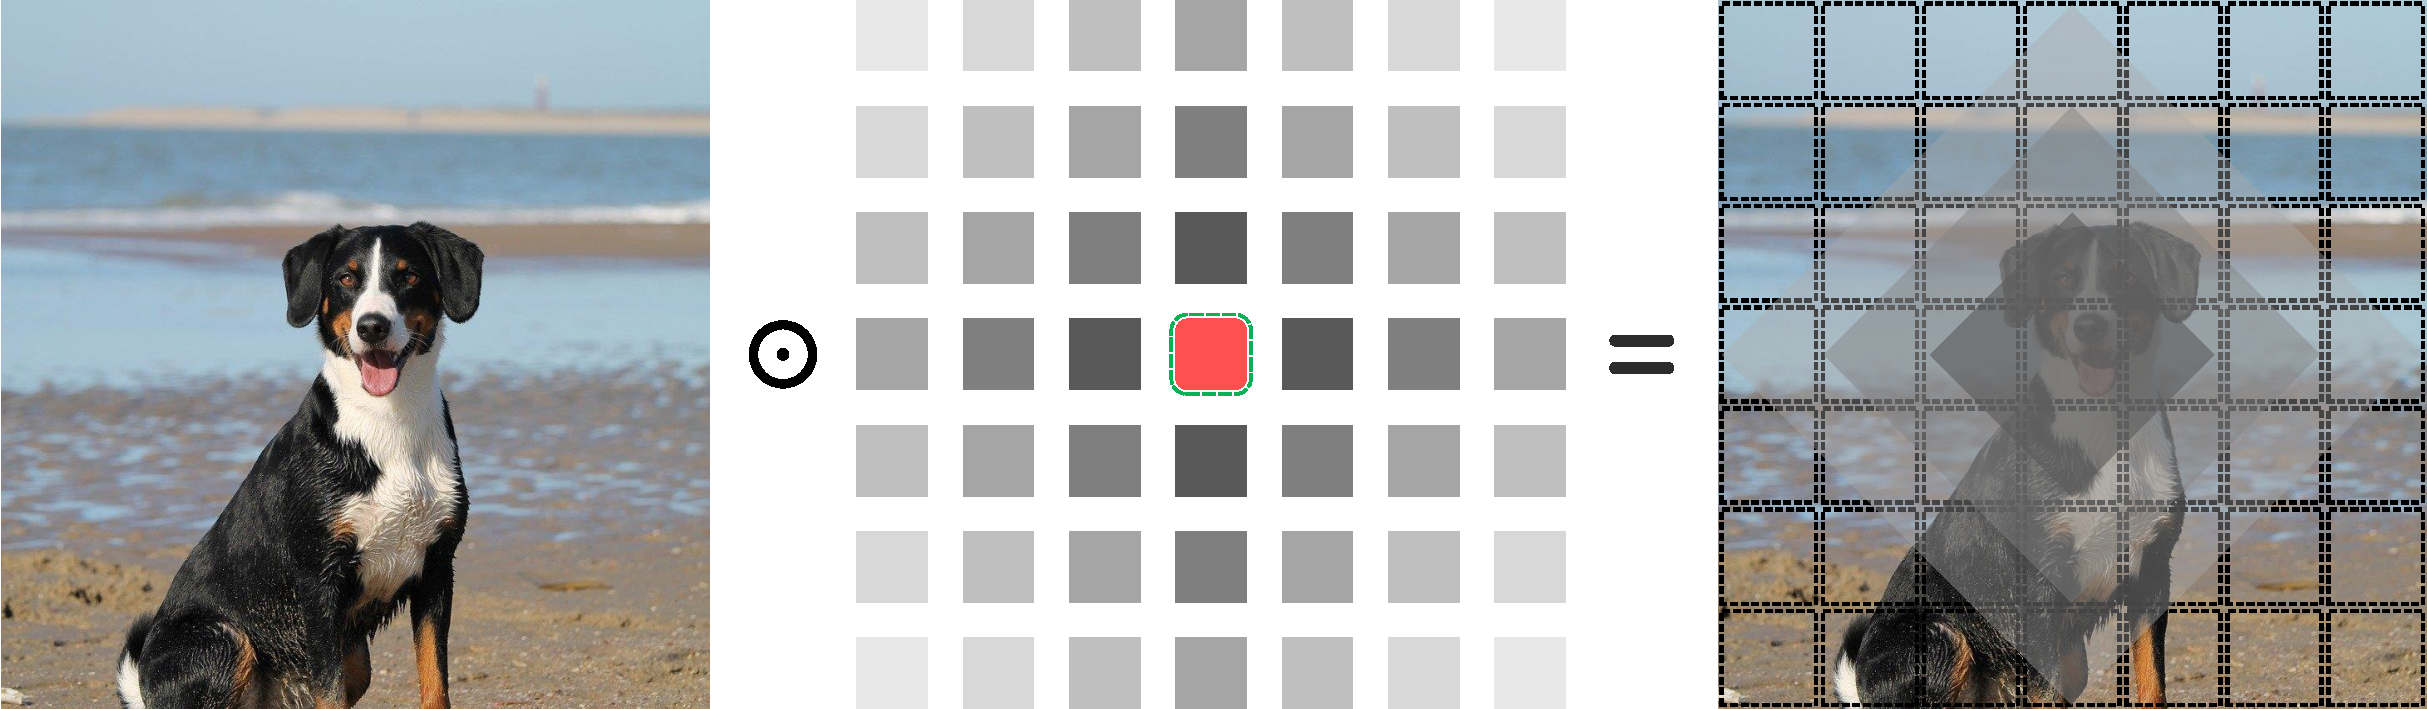
\includegraphics[width=0.9\textwidth]{./Img/空间衰减注意力.pdf}
  \caption{ESD:基于显式超先验的空间衰减注意力}\label{fig:4-5}
\end{figure}


其中 $\overline{\Theta}$ 是 $\Theta$ 的复共轭,$D\in \mathbb{R}^{|x|\times|x|}$ 包含因果掩蔽和指数衰减,它表示一维序列中的相对距离,并带来上下文数据的显式时间先验。受到 RetNet 一维显式时间先验思想的启发,我们创新性的设计了一种基于空间显式超先验的空间衰减注意机制(\textbf{ESD}),如图 \ref{fig:4-5} 所示,在上述并行化计算的基础之上,将其拓展为二维空间衰减注意机制。

在图像的上下文数据中,每个元素标记都通过平面内的二维坐标进行唯一定位,第 $n$ 个标记表示为 $(x_n, y_n)$。 为了适应这一点,需要调整矩阵 $D$ 中的每个元素,以基于其 $2D$ 坐标来表示各个标记对之间的空间相对距离。矩阵 $D$ 的计算公式如下:
\begin{align}
    D_{nm}^{2d}=\gamma^{|x_n-x_m|+|y_n-y_m|}
\end{align}

\begin{figure}[ht]
  \centering
  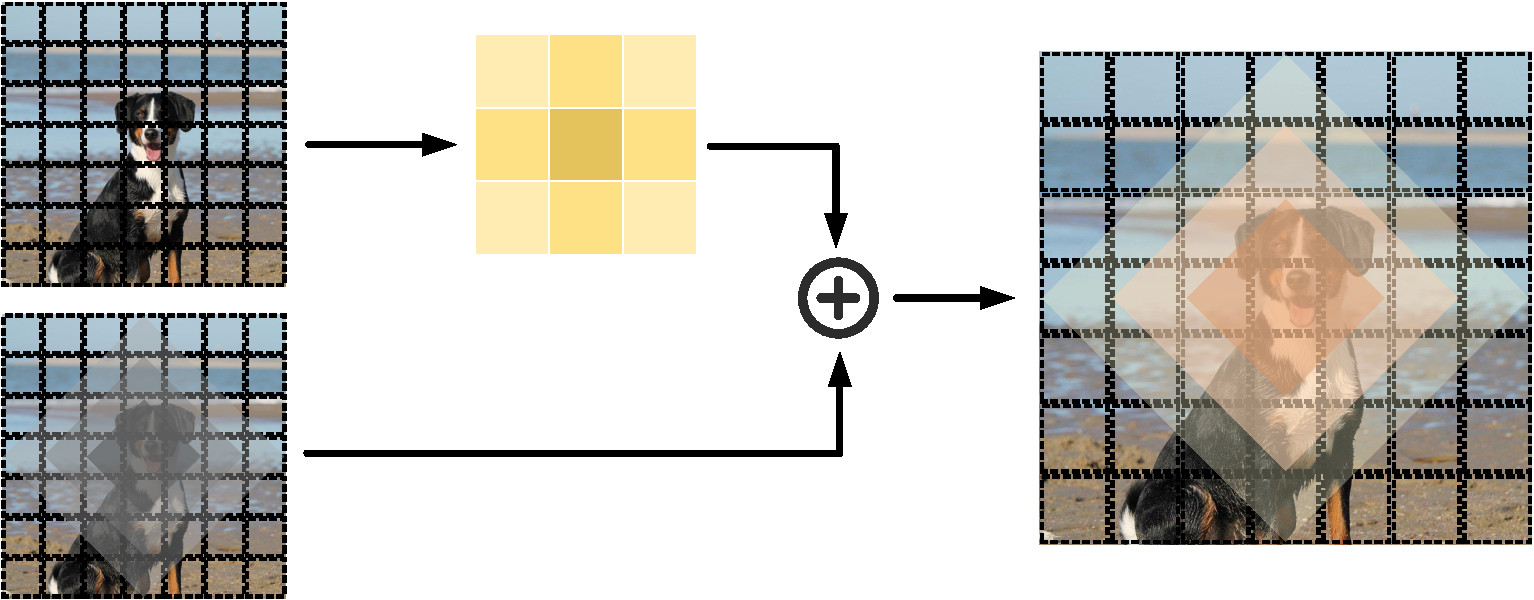
\includegraphics[width=0.876\textwidth]{./Img/输出结合.pdf}
  \caption{空间衰减注意力结合卷积增强得到最终输出}\label{fig:4-6}
\end{figure}


最后,引入 $\text{Softmax}(\cdot)$ 进行非线性操作,再结合上下文增强的卷积操作得到最终的输出,如图 \ref{fig:4-6},因此,完整的空间衰减注意机制的表达式为:
\begin{align}
    \mathrm{ESD}(X)&=(\mathrm{Softmax}(QK^{\mathsf{T}})\odot D^{2d})V\\
    D_{nm}^{2d}&=\gamma^{|x_{n}-x_{m}|+|y_{n}-y_{m}|} \\
    X_{out} &= \mathrm{ESD}(X)+\mathrm{Conv}(V)
\end{align}



\subsubsection{损失函数设计}

在本研究中,我们使用了基于二进制哈希学习的方法对于全局特征和局部特征进行哈希学习。对于 $q$ 个查询数据点,将其表示为 $\{q_i\}_{i=1}^q$,同时,对于 $p$ 个数据点,将其表示为 $\{p_i\}_{i=1}^p$。然后,针对每一对的 $q_i$ 和 $p_j$,将由一个全局特征 $v^{global}$ 和 $m$ 个局部特征 $v^{local}_i$ 组成,每一对的 $q_i$ 和 $p_j$ 对应的哈希码可以通过下面公式得到:
\begin{align}
    u_i=\operatorname{sign}(q_i) ,\quad z_j=\operatorname{sign}(p_j)
\end{align}

其中,$u_i,z_j\in\{-1,+1\}^k$,$k$ 代表着最终输出的二进制哈希码的长度。设 $F$ 表示模型中全局和局部特征学习的整合,$\mathrm{W}=\{\mathrm{W}^{global};\mathrm{W}_1^{local};\mathrm{W}_2^{local};\ldots;\mathrm{W}_m^{local}\}$为二进制代码映射模块,$\Theta$ 代表模型需学习的参数集。对于给定的输入图像 $I$,全局和局部特征学习整体输出如下:
\begin{align}
    O = \mathrm{W} \cdot F(I;\Theta)
\end{align}

然后,我们使用 $\text{tanh}(\cdot)$ 针对 $O$ 进行激活得到模型最终的输出 $O^\prime = \text{tanh}(O)$,最终的损失 $\mathcal{L}$ 设计如下:
\begin{align}
    \mathcal{L}_{\mathrm{W},\Theta}(I)=
        \alpha\sum_{i\in\Omega}\sum_{j\in\Gamma}\left[{O^\prime_i}^\top z_j-kS_{ij}\right]^2+\beta\sum_{i\in\Omega}\left[z_i-{O^\prime_i}\right]^2
    \label{eq:final_eq}
\end{align}

其中 $\alpha$ 和 $\beta$为网络训练时的权衡超参数,$\Gamma$ 代表所有数据库点的索引,而 $\Omega \subseteq \Gamma$ 表示查询集点的索引。$S \in \{-1,+1\}{}^{q \times p}$ 是一个监督矩阵,其值可以在模型训练过程中自动调整。在 LGESD 模型中,我们规定在每次计算损失时,数据库点与查询集点之间不能有共同的项,确保数据库和查询集之间保持互补关系。

\subsubsection{实验过程设计}

\textbf{数据集划分}:本研究在四个数据集上进行,分别是CUB200-2011 \cite{Wah2011TheCB}、Aircraft \cite{maji2013finegrained}、Food101 \cite{food101_2014} 以及 NABirds \cite{nabirds2015},其中 CUB200-2011 和 Aircraft 属于广泛使用的数据集,Food101 和 NABirds 属于流行的大规模细粒度数据集。CUB200-2011 为鸟类数据集,包含了200种鸟类的11788张图像,我们将其分为5994张图像用于训练,5794张图像用于测试。Aircraft 为飞机数据集,包含了100种类型飞机的10000张图像,将其中6667张图像用于训练,3333张图像用于测试。Food101 为具有101000张图像的101种食品类数据集,每个类别中有1000张图像,我们按照每个类别挑选750张图像用于训练,250张用于测试,划分出训练图像75750张,测试图像25250张。NABirds 包含了48562张图像的北美鸟类数据集,其中555种北美子鸟类,我们将23929张图像用于训练,24633种图像用于测试。

\textbf{训练设置}:对于CUB200-2011、Aircraft 以及 Food101 三个数据集,我们设置每个 Epoch 随机采样的样本数为2000个,而对于 NABirds 数据集,设置每个 Epoch 随机采样的样本数为 4000 个。对于所有的数据集,我们设定每张输入的图像预处理为 $224 \times 224$ 大小,训练次数 Epoch 为30次,设定迭代时间为 50,迭代的学习率设置为 $5 \times 10^{-4}$,批量的大小设置为 16,使用 SGD 作为优化器,骨干网络选择 ResNet-50 \cite{he2015deep},训练过程的权重衰减和动量分别设置为 $10^{-4}$ 和 $0.91$。在公式 \ref{eq:final_eq} 中的 $\alpha$ 和 $\beta$ 我们分别设置为 $0.6$ 和 $30$。在公式 \ref{eq:eq_4_m} 中的 $m$ 我们设置为3,因此最终的全局和局部双轨结构的输出哈希码长度分别为 $\frac{k}{2}$ 和 $\frac{k}{6}$,其中 $k$ 为训练时指定的最终输出的哈希码的长度。



\subsubsection{实验执行结果}


\begin{figure}[h]
  \centering
  \begin{subfigure}{0.48\textwidth}
    \centering
    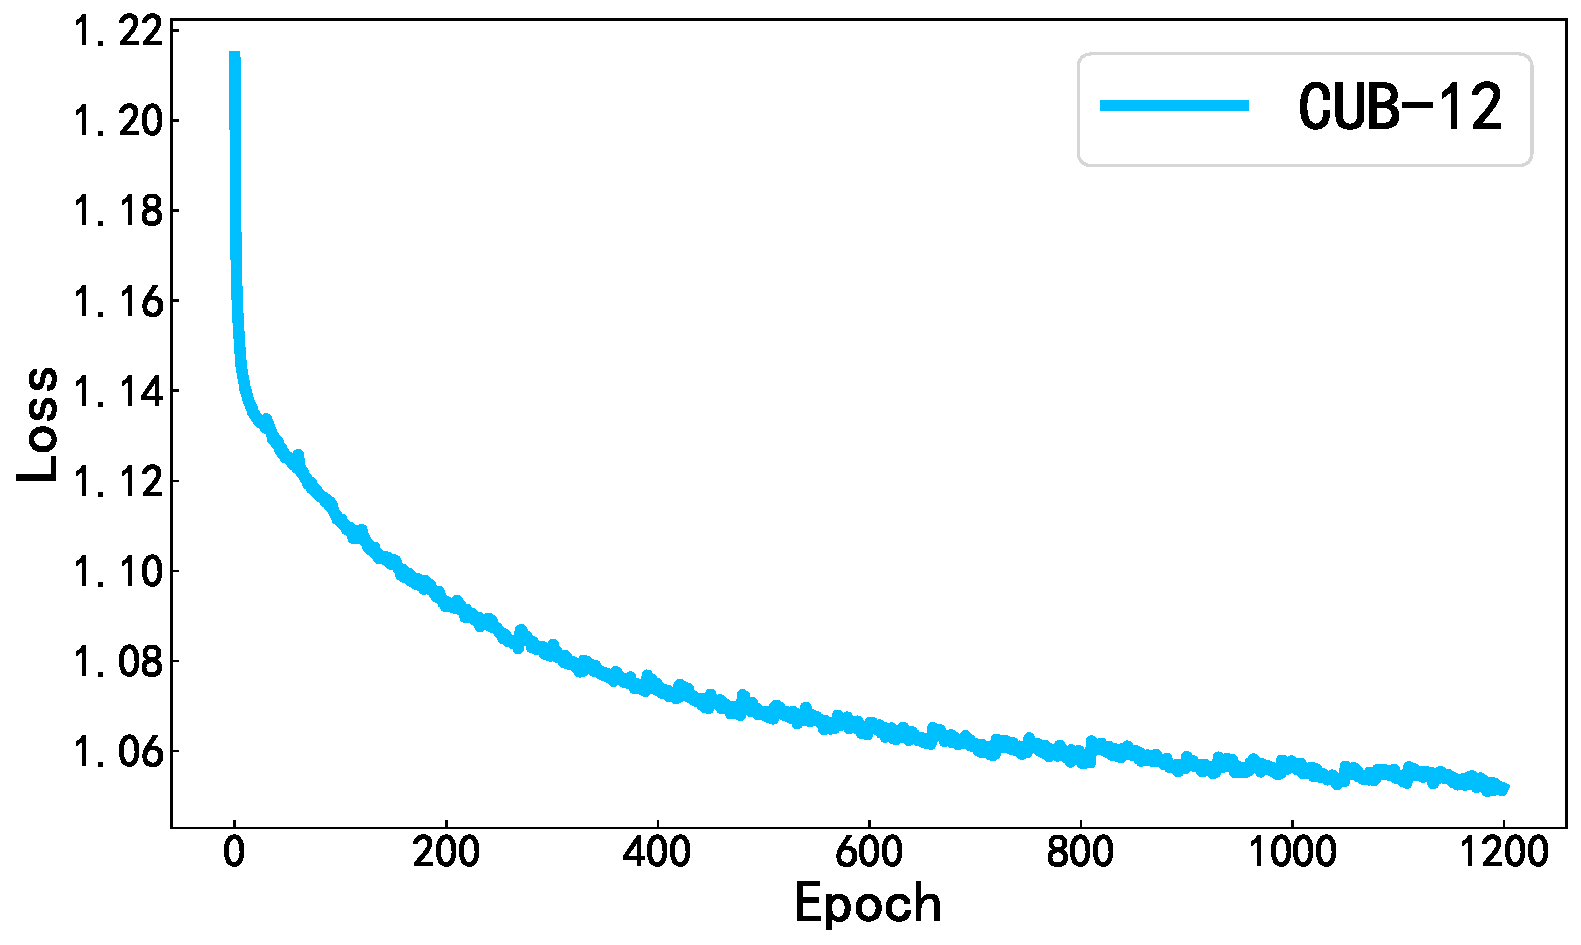
\includegraphics[width=\linewidth]{./Img/CUB-12.pdf}
    \caption{$k=12$}\label{fig:4-24}
  \end{subfigure}
  \hfil
  \begin{subfigure}{0.48\textwidth}
    \centering
    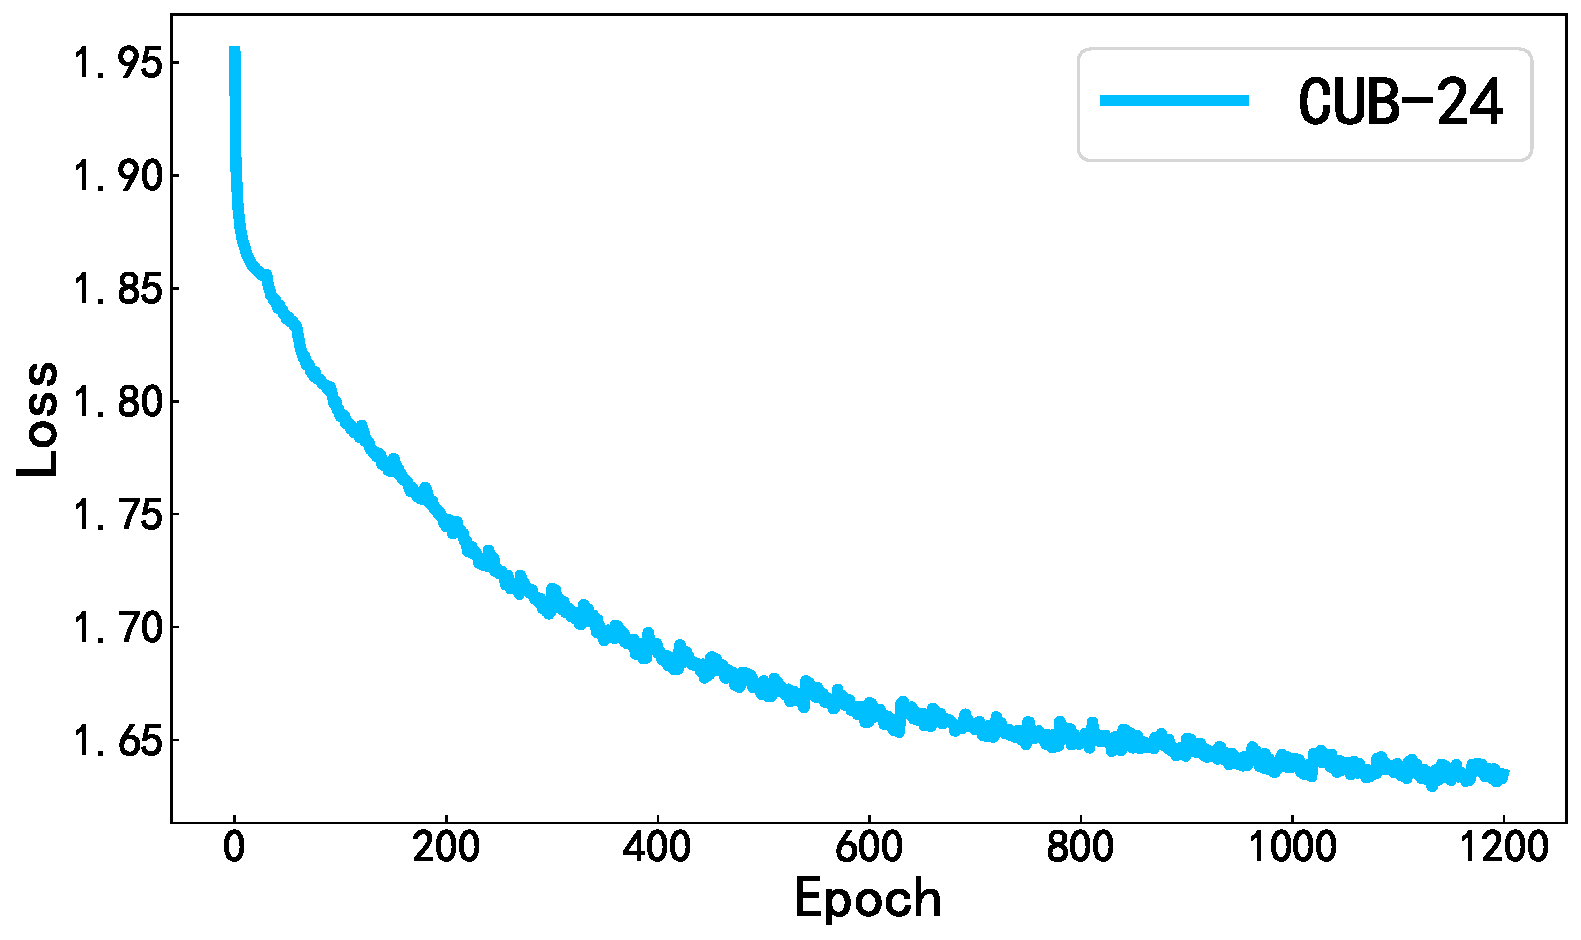
\includegraphics[width=\linewidth]{./Img/CUB-24.pdf}
    \caption{$k=24$}\label{fig:4-25}
  \end{subfigure}
  \hfil
  \begin{subfigure}{0.48\textwidth}
    \centering
    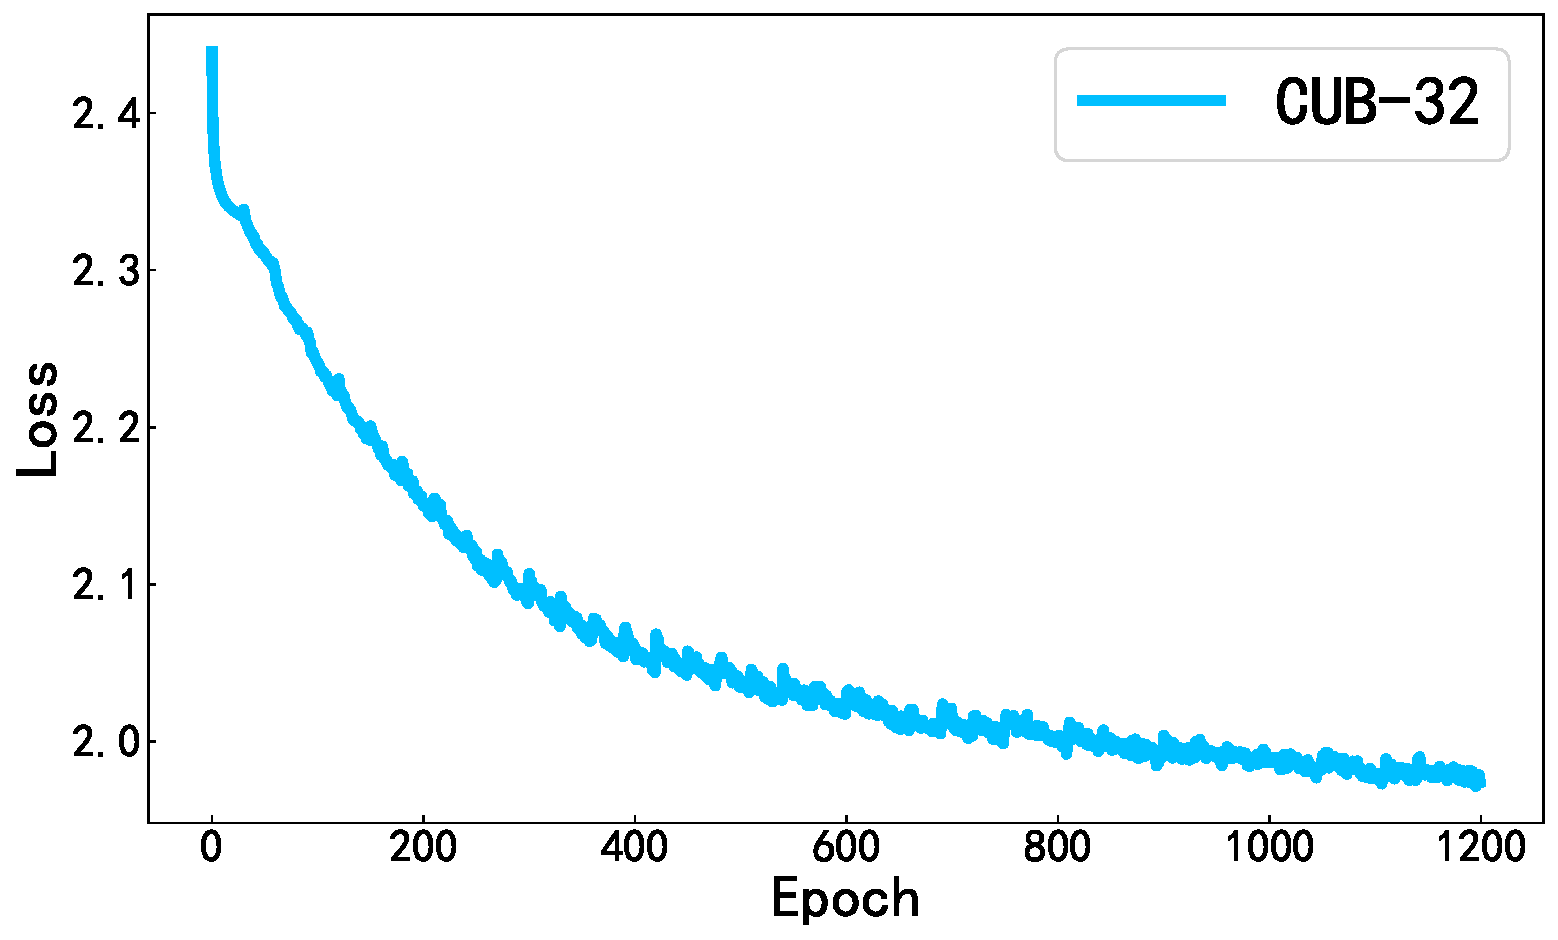
\includegraphics[width=\linewidth]{./Img/CUB-32.pdf}
    \caption{$k=32$}\label{fig:4-26}
  \end{subfigure}
  \hfil
  \begin{subfigure}{0.48\textwidth}
    \centering
    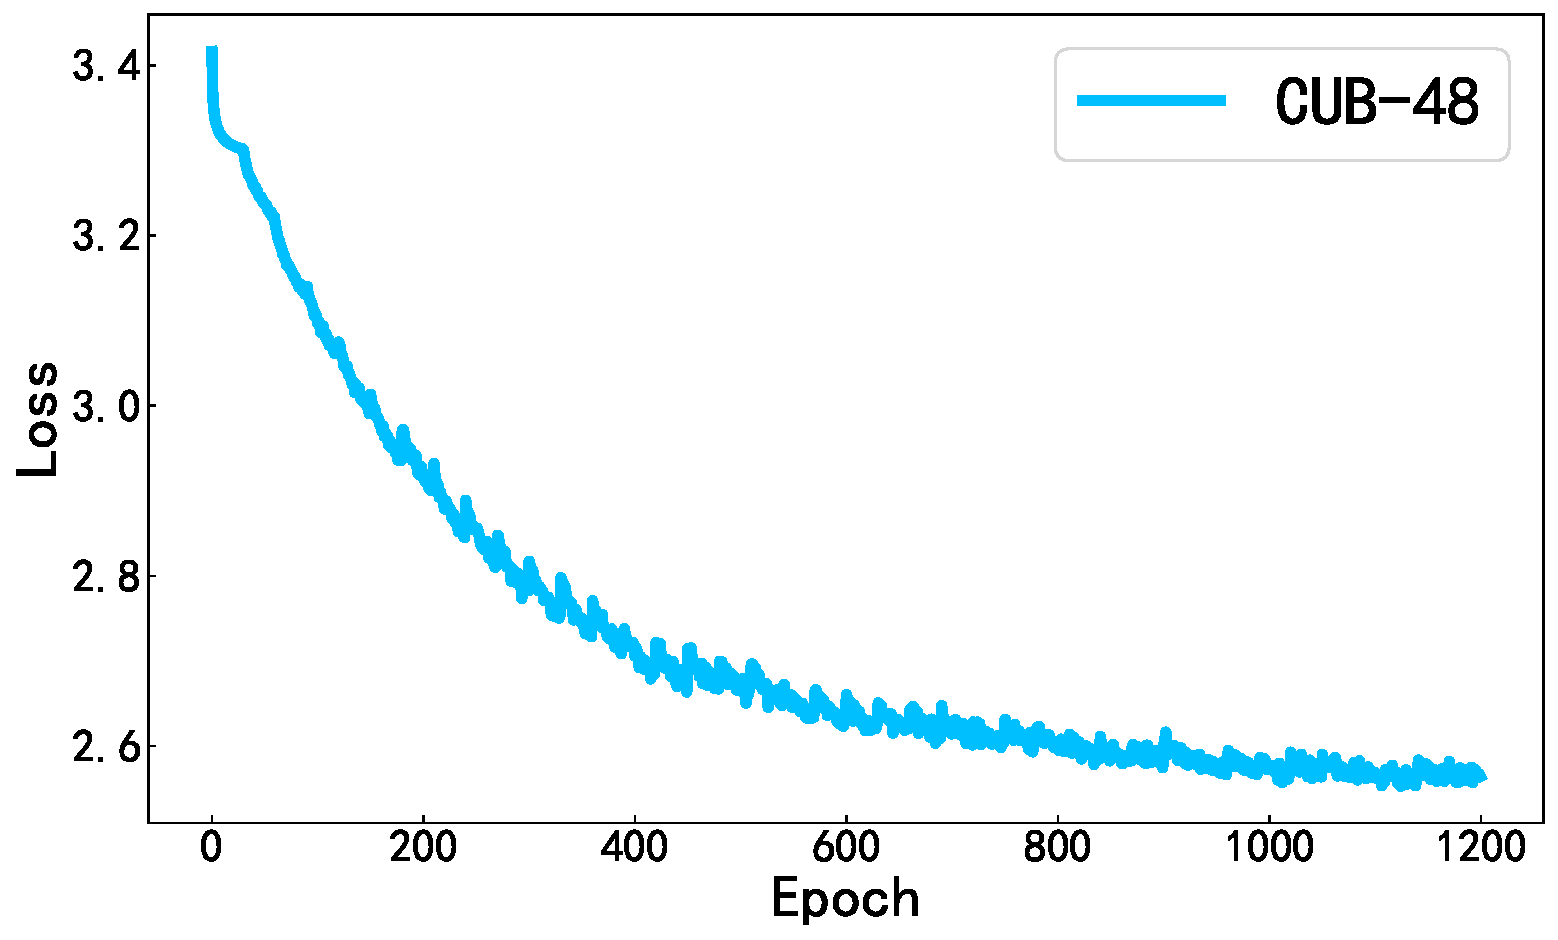
\includegraphics[width=\linewidth]{./Img/CUB-48.pdf}
    \caption{$k=48$}\label{fig:4-27}
  \end{subfigure}
  \caption{CUB200-2011数据集的12-48哈希码长度训练损失}
  \label{fig:4-28}
\end{figure}

如图 \ref{fig:4-24} 至 \ref{fig:4-27} 所示,这一系列四幅图表详尽描绘了LGESD在同个数据集的不同哈希码长度上的训练进程中,损失函数的演变轨迹。当哈希码长度为32时,损失值从初始的2.4稳步下探至约2.0,直观展示了模型效能的稳步提升。类似地,哈希码长度为12的训练轨迹亦呈现出乐观的下降态势,损失值由1.22优化至1.06,再度验证了模型在迭代学习中的持续优化能力。在采用48位哈希码的配置下,因编码长度的增益,模型被赋予了学习更为复杂和丰富的特征表达空间的能力,进而导致初期损失值设定于较高水平(3.0)。然而,随着训练进程的推移,这一数值稳步下滑至约2.6,并呈现平稳趋势,这一动态不仅揭示了模型在克服初期高挑战起点时的韧性,还显著证明了其在应对高级分类任务时的学习效率与灵活适应性。综观所有实验情境,随着训练次数(Epoch)的累加,损失函数的递减速率渐趋缓慢,标志着模型学习已逼近收敛状态,实现了训练目标。

模型训练完成之后,我们针对模型进行平均预测精度(mAP)评估,得到的结果如表 \ref{tab:experiments} 所示,在对四个关键数据集的深入剖析中,LGESD展示出相对于A${}^2$-Net持续且明显的优越性。具体到CUB200-2011数据集,LGESD从采用12位哈希码起始,即以41.50\%的mAP成绩奠定了领先地位,此时A${}^2$-Net为33.83\%;而随着哈希长度扩展至48位,LGESD的mAP显著跃升至80.12\%,与A${}^2$-Net的77.33\%形成对比,进一步凸显其优势。转观Aircraft数据集,这种优势在12至32位的哈希码范围内尤为突出,LGESD从50.37\%逐步攀高至85.06\%的峰值,相比之下,A${}^2$-Net在同一区间的表现由42.72\%增长至81.37\%,虽有进步,但仍略逊一筹。在food101与NABirds这两个数据集的探索中,无论哈希长度如何变化,LGESD均稳固保持其领先地位,不断验证其在多样化任务中的高效性能与适应力。

\begin{table*}[t]
	\caption{LGESD模型的平均预测精度(\%mAP)与现有方法对比}
	\label{tab:experiments}
	\centering
	\resizebox{1.0\linewidth}{!}{
	\begin{tabular}{c|c|cccccccccc}
		\toprule
		数据集 & 哈希码长度 & ITQ & SDH & DPSH & HashNet & ADSH & ExchNet & A${}^2$-Net & \textbf{LGESD}\\		
		\midrule
		\multirow{4}{*}{CUB200-2011}
            &$k=12$&6.80&10.52&8.68&12.03&20.03&25.14&33.83     &  \textbf{41.50}   \\
            &$k=24$&9.42&16.95&12.51&17.77&50.33&58.98&61.01    &  \textbf{67.33}   \\
            &$k=32$&11.19&20.43&12.74&19.93&61.68&67.74&71.61   &  \textbf{74.01}   \\
            &$k=48$&12.45&22.23&15.58&22.13&65.43&71.05&77.33   &  \textbf{80.12}   \\
		\hline
    	\multirow{4}{*}{Aircraft}  
            &$k=12$&4.38&4.89&8.74&14.91&15.54&33.27&42.72      &  \textbf{50.37}   \\
            &$k=24$&5.28&6.36&10.87&17.75&23.09&45.83&63.66     &  \textbf{76.61}   \\
            &$k=32$&5.82&6.90&13.54&19.42&30.37&51.83&72.51     &  \textbf{81.49}   \\
            &$k=48$&6.05&7.65&13.94&20.32&50.65&59.05&81.37     &  \textbf{85.06}   \\
		\hline
		\multirow{4}{*}{Food101}          
            &$k=12$&6.46&10.21&11.82&24.42&35.64&45.63&46.44    &  \textbf{52.16}   \\
            &$k=24$&8.20&11.44&13.05&34.48&40.93&55.48&66.87    &  \textbf{77.71}   \\
            &$k=32$&9.70&13.36&16.41&35.90&42.89&56.39&74.27    &  \textbf{81.05}   \\
            &$k=48$&10.07&15.55&20.06&39.65&48.81&64.19&82.13   &  \textbf{83.20}   \\
		\hline
		\multirow{4}{*}{NABirds}           
            &$k=12$&2.53&3.10&2.17&2.34&2.53&5.22&8.20          &  \textbf{8.96}    \\
            &$k=24$&4.22&6.72&4.08&3.29&8.23&15.69&19.15        &  \textbf{21.34}   \\
            &$k=32$&5.38&8.86&3.61&4.52&14.71&21.94&24.41       &  \textbf{28.64}   \\
            &$k=48$&6.10&10.38&3.20&4.97&25.34&34.81&35.64      &  \textbf{41.88}   \\
		\bottomrule
	\end{tabular}}
\end{table*}

\subsubsection{实验结果分析}

\begin{figure}[h]
  \centering
  \begin{subfigure}{0.48\textwidth}
    \centering
    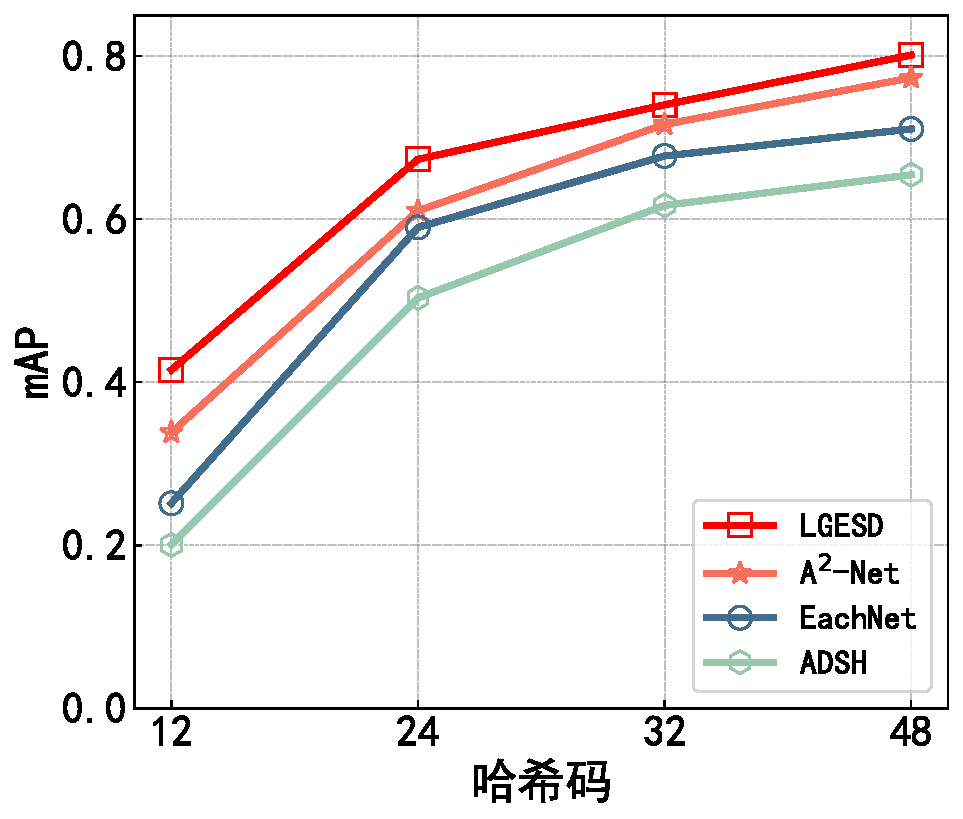
\includegraphics[width=\linewidth]{./Img/CUB-R50.pdf}
    \caption{基于CUB200-2011数据集的mAP对比}\label{fig:4-29}
  \end{subfigure}
  \hfil
  \begin{subfigure}{0.48\textwidth}
    \centering
    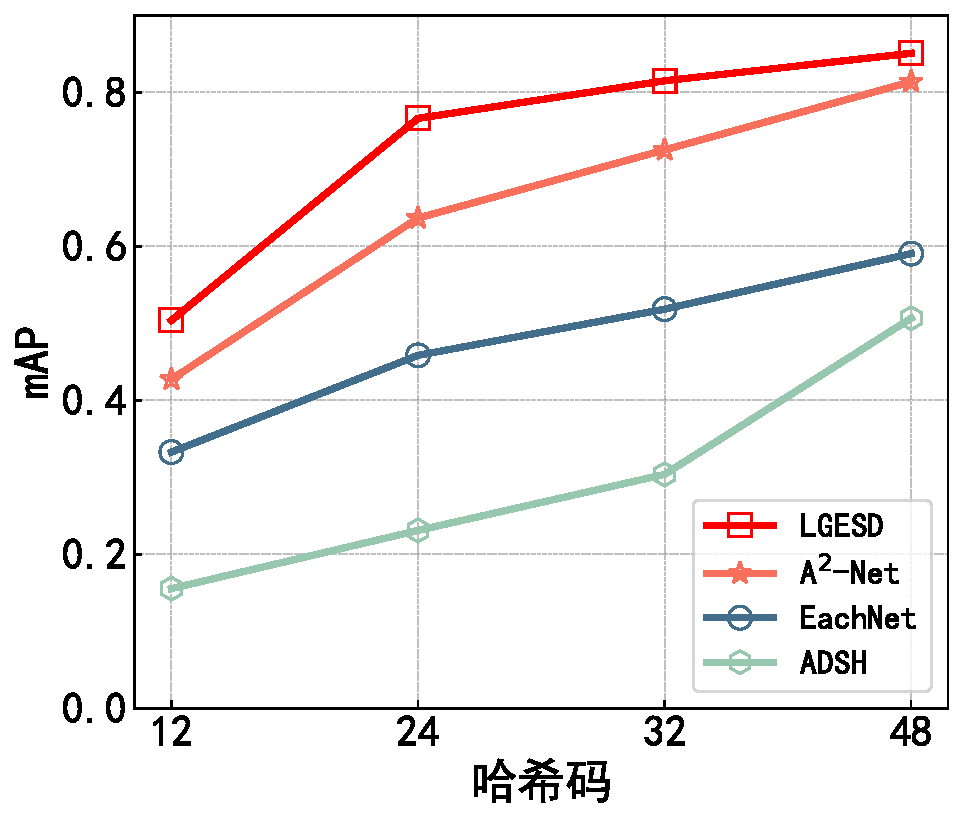
\includegraphics[width=\linewidth]{./Img/Aircraft-R50.pdf}
    \caption{基于Aircraft数据集的mAP对比}\label{fig:4-30}
  \end{subfigure}
  \hfil
  \begin{subfigure}{0.48\textwidth}
    \centering
    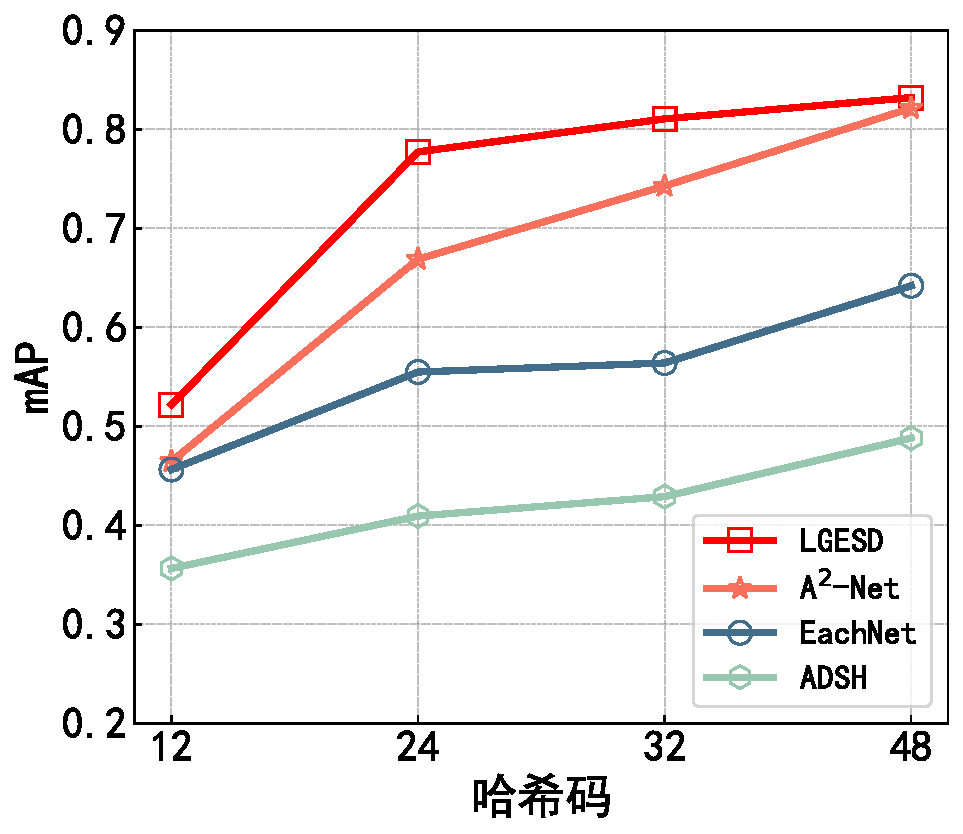
\includegraphics[width=\linewidth]{./Img/Food-R50.pdf}
    \caption{基于Food101数据集的mAP对比}\label{fig:4-31}
  \end{subfigure}
  \hfil
  \begin{subfigure}{0.48\textwidth}
    \centering
    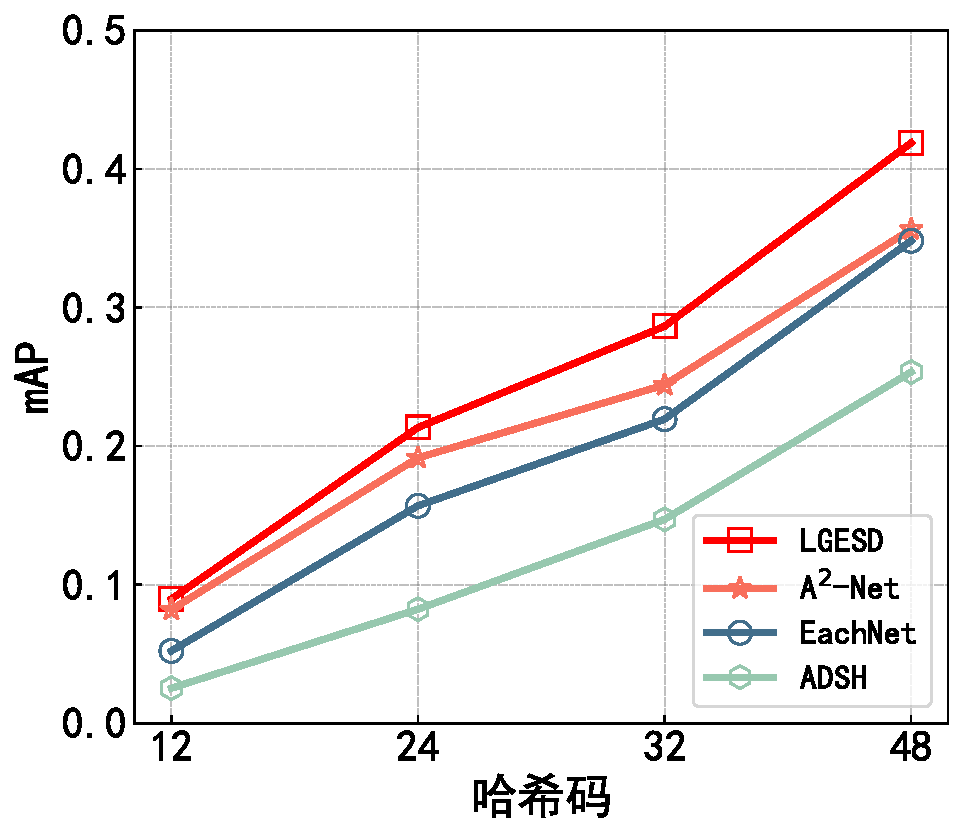
\includegraphics[width=\linewidth]{./Img/Nabirds-R50.pdf}
    \caption{基于NABirds数据集的mAP对比}\label{fig:4-32}
  \end{subfigure}
  \caption{LGESD与现有方法在四个数据集上的mAP对比}
  \label{fig:4-32-a}
\end{figure}

为了更清晰的显示LGESD模型较现有方法的mAP提升,我们选择了 LGESD、A${}^2$-Net、EachNet以及ADSH四个方法的12-48哈希码长度进行可视化显示,如图 \ref{fig:4-32-a} 所示,从两个图当中可以看出,LGESD算法模型在哈希码长度变化的影响分析中展现了一种明确的正向发展趋势。随着哈希码长度的逐渐增加,LGESD的平均准确率(mAP)显著提升,这直接反映了哈希码长度与其识别和分类性能之间的正比关系。该特性表明,LGESD算法能够有效利用更长的哈希码来编码更多的输入信息,从而提升其在任务中的表现。这种对哈希码长度增加的敏感性和高效利用,不仅是算法设计合理性的体现,也是其在实践中可能获得更优解的关键因素之一。因此,在资源允许的情况下,针对LGESD模型选择更长的哈希码长度将是一个提升系统性能的有效策略。


\begin{figure}[h]
  \centering
  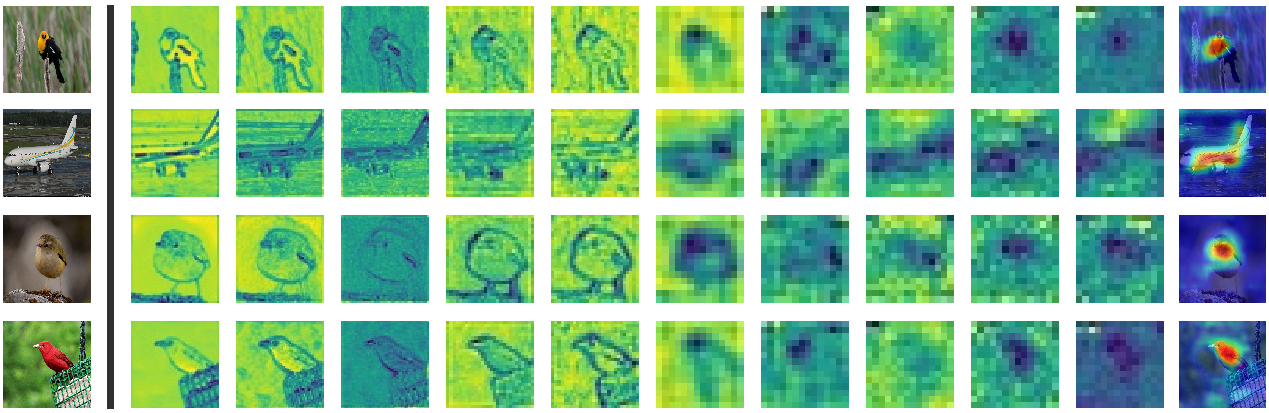
\includegraphics[width=1.0\textwidth]{./Img/中间层特征图.pdf}
  \caption{中间层特征图与注意力热图}\label{fig:4-20}
\end{figure}

图 \ref{fig:4-20} 展示了LGESD模型的训练过程,其中包括输入图像、中间层卷积特征以及注意力热图。从每一行图像的最后一个注意力热图中可以看出,LGESD模型成功地将注意力聚焦在了有效的对象上。这意味着模型能够准确地识别和关注图像中的关键区域,这对于提高模型的性能和准确性非常重要。通过这种集中的注意力,模型能够更好地理解图像内容,并在后续的处理过程中做出更准确的决策。这种成功的注意力聚焦表明模型在训练过程中取得了良好的效果,具备一定的能力处理复杂任务。

\begin{figure}[h]
  \centering
  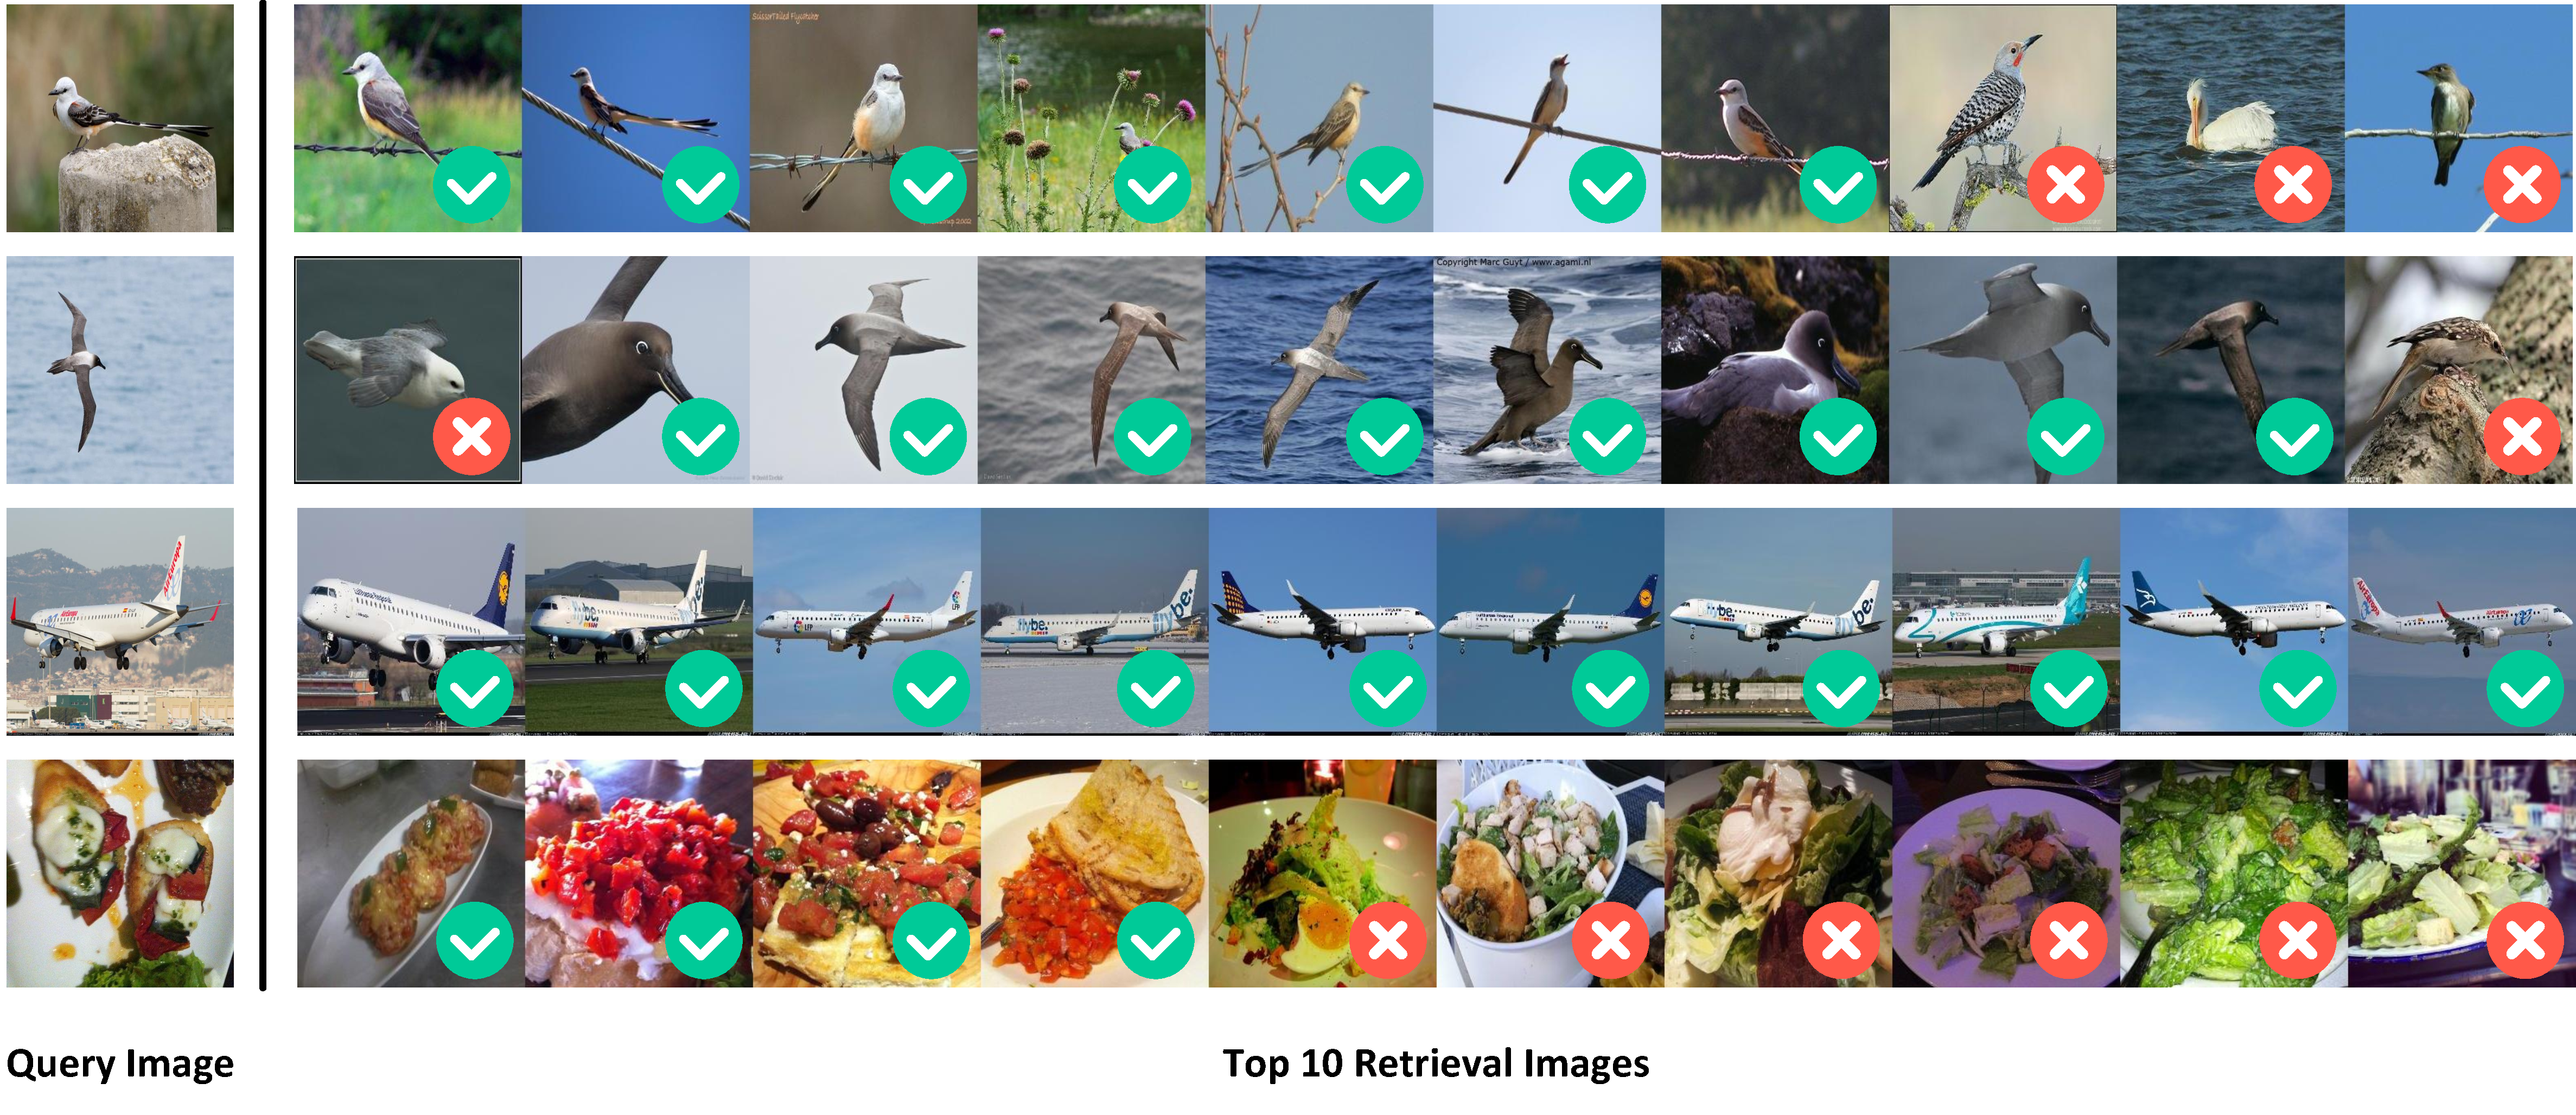
\includegraphics[width=1.0\textwidth]{./Img/最终检索图.pdf}
  \caption{LGESD模型的图像检索效果}\label{fig:4-33}
\end{figure}


在完成模型的训练和损失函数分析之后,我们进一步对模型进行了图像检索能力的测试。测试过程包括随机选取一张未知图像,将其作为查询输入到训练好的模型中。模型基于学习到的特征表示,对数据库中的图像进行排序,以找出与查询图像最相关的图像。我们收集了检索结果中排名最前的前十张图像,并进行了可视化展示。

具体来说,测试中我们首先从图像库中随机抽取了一张未参与训练的图像。随后,该图像被输入至模型,模型随即输出了与其最为相似的一系列图像。这些图像根据与查询图像的相似度得分进行排序,得分最高的图像排在最前。我们选择了排名前十的图像,并将它们与查询图像一起进行了可视化展示,以便于直观评估模型的检索效果,最终得到的可视化结果如图 \ref{fig:4-33} 所示。

在检索结果的前十名中,大多数图像都能正确地识别出与查询图像相同的类别。这一结果表明,模型在图像特征学习和相似性度量方面表现出了较高的准确性和可靠性。然而,尽管前十的检索结果中大部分都正确识别出了对应的类别,但仍有部分图像的识别结果有待提高。这提示我们在未来的工作中需要进一步优化模型的检索性能,可能通过改进特征提取算法、增加训练数据的多样性、调整模型参数等方式来实现。
























